\documentclass[11pt, letterpaper]{article}

\usepackage[utf8]{inputenc}
\usepackage[spanish, es-tabla]{babel}
\usepackage{amsmath}
\usepackage{amsfonts}
\usepackage{amssymb}
\usepackage[margin=2.5cm]{geometry}
\usepackage{graphicx}
\usepackage{float}
\usepackage{booktabs}
\usepackage[hidelinks]{hyperref}

\setlength{\parskip}{0.5em}
\setlength{\parindent}{0pt}

\title{
    \vspace{1cm}
    \Large \textbf{Tarea 2: Fundamentos de Procesamiento de Imagenes IEE2714}
}
\author{\textbf{Adrian Godoy}}

\begin{document}
\maketitle

\begin{center}
    Repositorio: \url{https://github.com/adrianalessandro/fundamendos_img_tarea_2}
\end{center}

\vspace{0.5cm}
\hrule
\vspace{0.5cm}

\section{Pregunta 1}
\subsection{Imagen sintetica y ruido Poisson}

Se construye una imagen de tamano $256\times256$ con tres regiones:
un fondo de intensidad $0.15$, un cuadrado centrado de $128\times128$
pixeles con intensidad $0.45$ y un circulo centrado de radio $32$ pixeles
con intensidad $0.80$. Las regiones se realizan mediante mascaras
disjuntas, incluyendo los pixeles cercanos a las fronteras.

El ruido se genera con:
\[
y=\frac{\operatorname{Poisson}(N x)}{N}, \qquad N=40,
\]
La desviacion estandar observada del ruido aumenta con la intensidad: fue
aproximadamente $0.0614$ en el fondo, $0.1062$ en el cuadrado y $0.1436$ en
el circulo.

\begin{figure}[H]
    \centering
    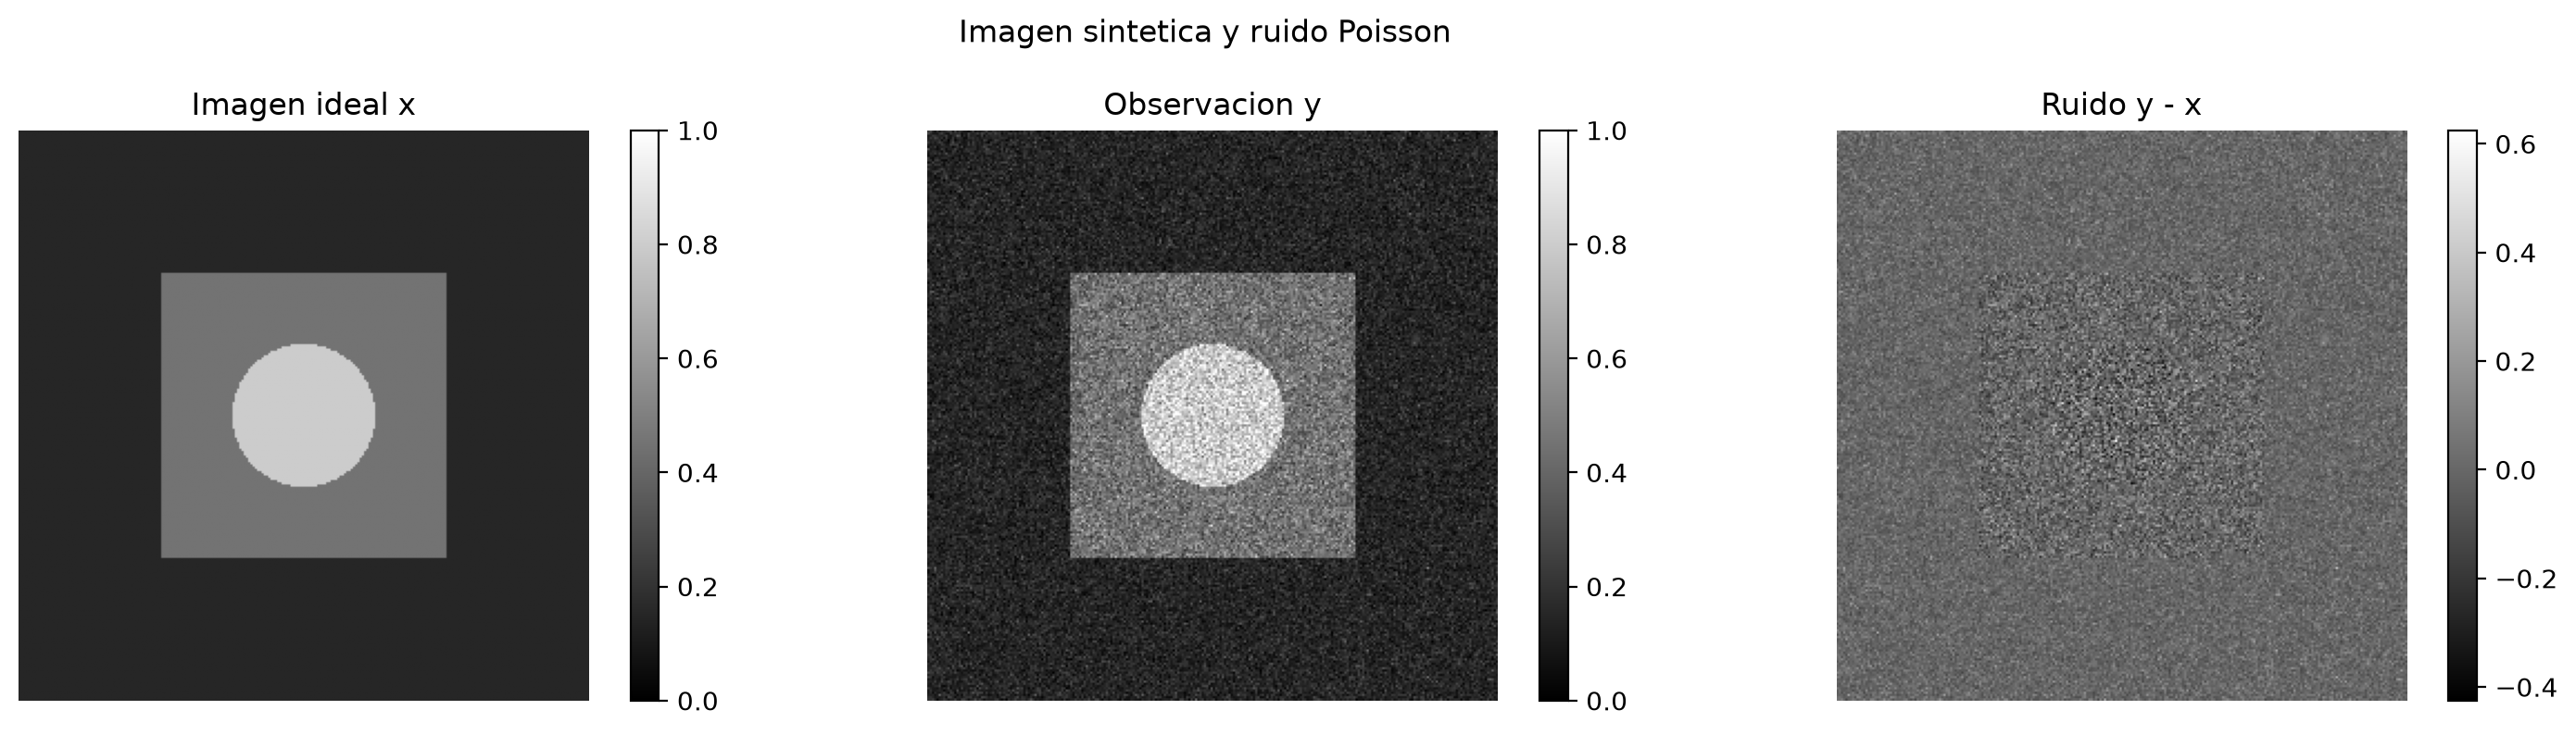
\includegraphics[width=0.95\textwidth]{pregunta_1/output/imagen_sintetica_ruido_poisson.png}
    \caption{Imagen ideal, observacion con ruido Poisson y ruido agregado.}
\end{figure}

\subsection{Implementacion del filtro Gaussiano}

El kernel Gaussiano isotropico se construye a partir de un valor real de
$\sigma$. Para limitar el costo, se uso un soporte de tres desviaciones
estandar:
\[
r=\lceil 3\sigma\rceil,
\qquad
K(i,j)=\exp\left(-\frac{i^2+j^2}{2\sigma^2}\right),
\quad i,j\in[-r,r].
\]
Finalmente, el kernel se normaliza dividiendo cada coeficiente por la suma
total. De esta forma, una region constante conserva aproximadamente su
intensidad despues del filtrado. La convolucion se realizo con extension
reflectiva en los bordes.

\begin{figure}[H]
    \centering
    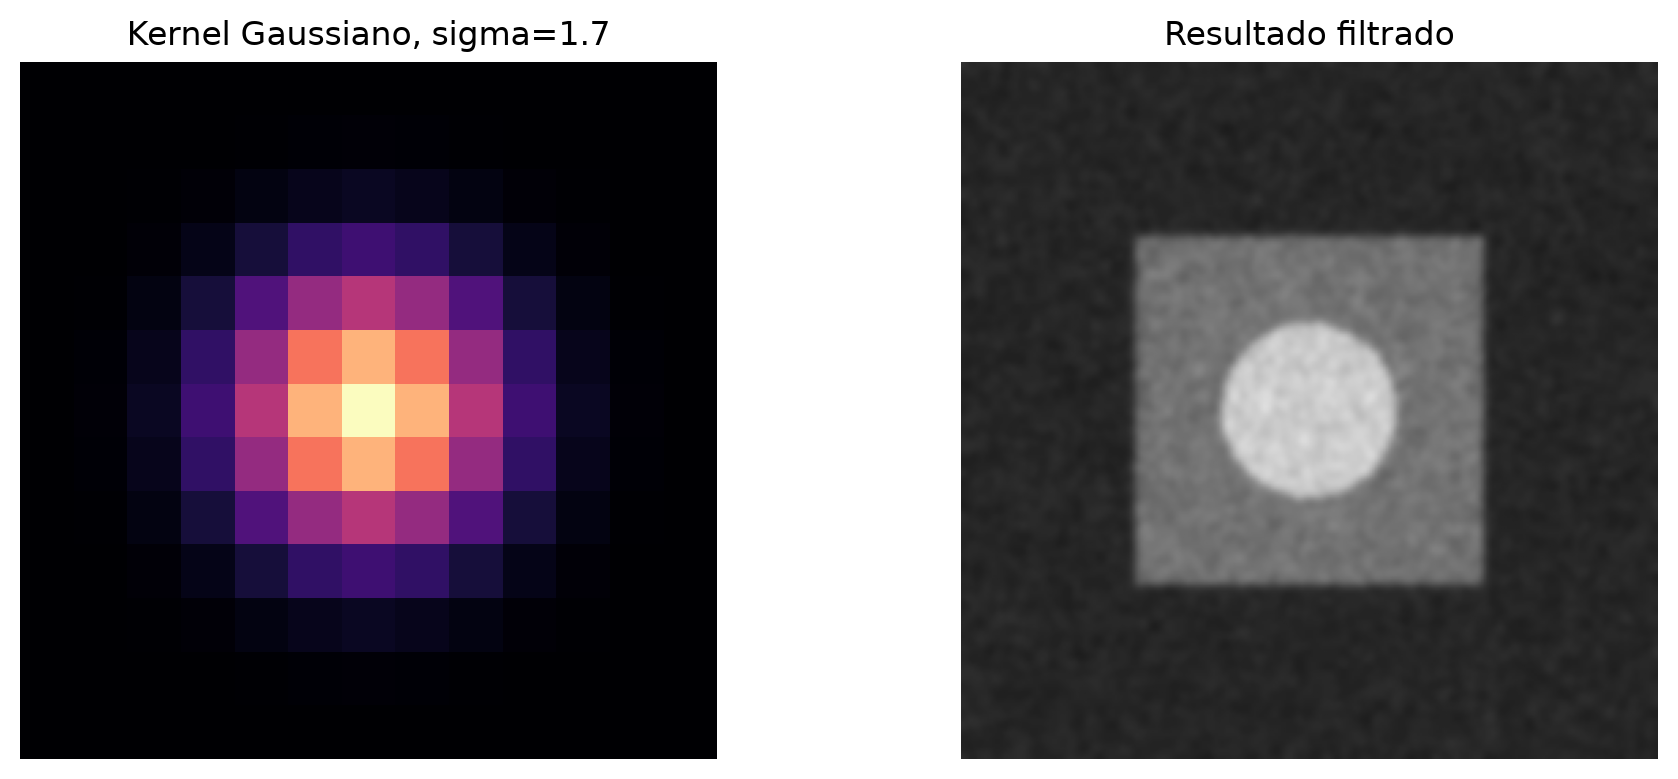
\includegraphics[width=0.75\textwidth]{pregunta_1/output/implementacion_kernel_gaussiano.png}
    \caption{Kernel Gaussiano construido con $\sigma=1.7$ y resultado del filtrado.}
\end{figure}

\subsection{Experimentacion y analisis}

Se evalua el caso sin filtrado y un rango denso de valores de $\sigma$ entre
$0.25$ y $8$. Para cada valor se calculo el RMSE global y el RMSE dentro de
cada mascara. Los minimos obtenidos fueron:

\begin{table}[H]
    \centering
    \begin{tabular}{lcc}
        \toprule
        Region & $\sigma$ optimo & RMSE minimo \\
        \midrule
        Fondo & 1.849 & 0.016567 \\
        Cuadrado sin circulo & 1.357 & 0.036869 \\
        Circulo & 1.480 & 0.043401 \\
        Global & 1.480 & 0.024104 \\
        \bottomrule
    \end{tabular}
    \caption{Valores optimos obtenidos en el barrido de $\sigma$.}
\end{table}

No existe un mismo $\sigma$ que minimice simultaneamente las tres regiones.
El fondo tiene menor ruido absoluto, mientras que el circulo tiene mayor
ruido. Ademas, las mascaras incluyen zonas cercanas a bordes, donde un kernel
grande mezcla intensidades distintas y genera sesgo. Por esto, el error no
depende solamente del nivel de ruido, sino tambien de la cantidad de
fronteras presentes en la region.

\begin{figure}[H]
    \centering
    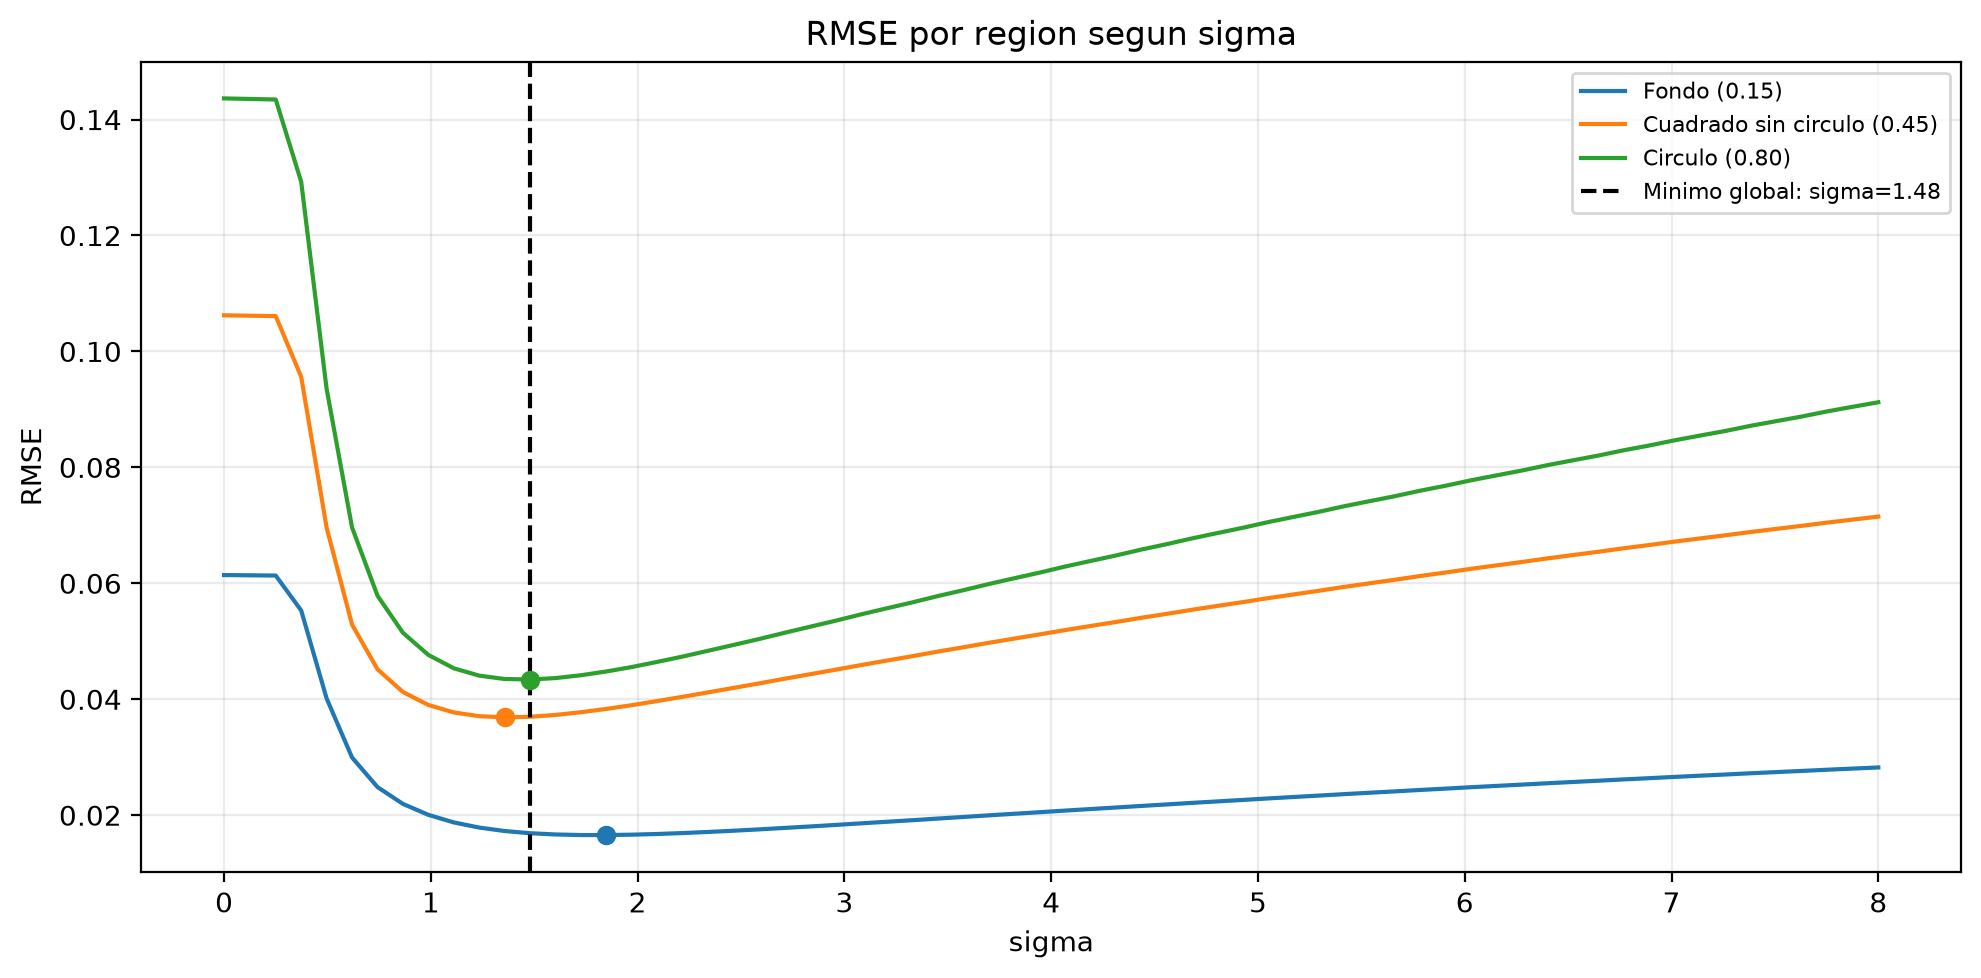
\includegraphics[width=0.78\textwidth]{pregunta_1/output/experimentacion_rmse_sigma.png}
    \caption{RMSE de cada region en funcion de $\sigma$.}
\end{figure}

\begin{figure}[H]
    \centering
    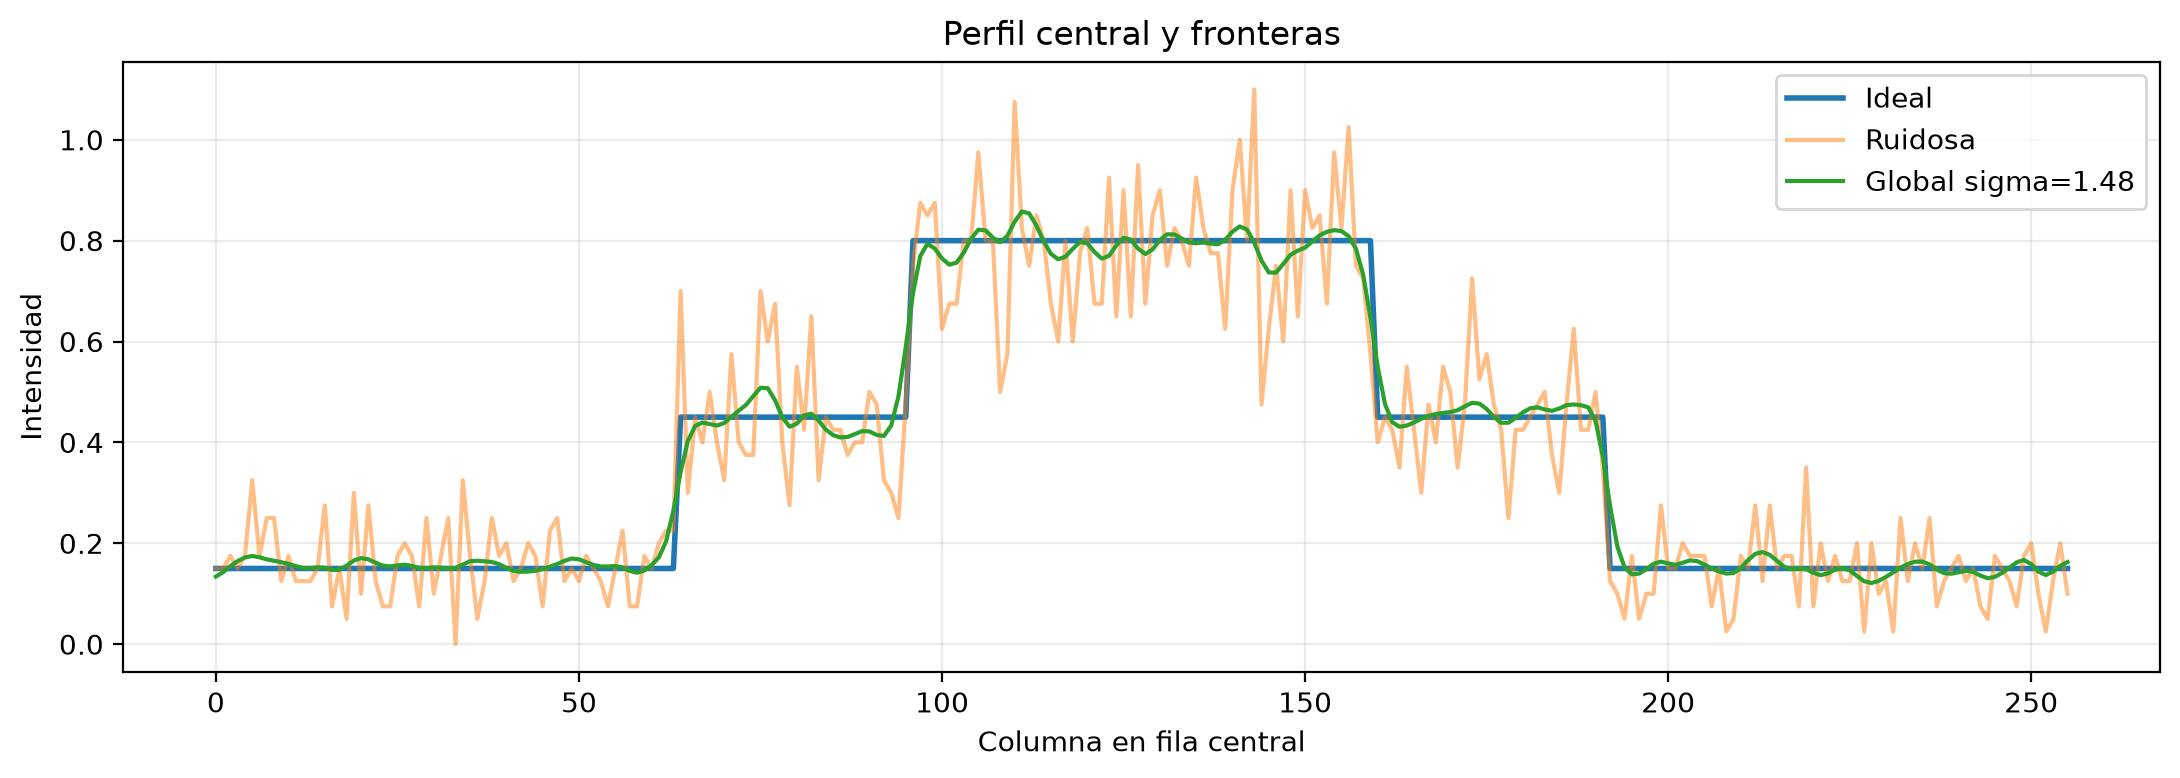
\includegraphics[width=0.85\textwidth]{pregunta_1/output/experimentacion_perfil_frontera.png}
    \caption{Perfil central de la imagen y efecto del filtrado en las fronteras.}
\end{figure}

\subsection{Filtro espacialmente adaptativo}

Para adaptar el filtro se estimo primero una intensidad local
$\hat{\mu}(x,y)$ aplicando un suavizado Gaussiano auxiliar con
$\sigma_{\mathrm{aux}}=2$. Luego se definio una regla por interpolacion
lineal a partir de los optimos regionales:
\[
(0.15,1.849), \qquad (0.45,1.357), \qquad (0.80,1.480).
\]
Cada valor de $\hat{\mu}(x,y)$ se transformo en un valor
$\sigma(x,y)$ mediante esta interpolacion. Para aproximar el filtro variable
se calcularon respuestas con los tres sigmas nodales y se mezclaron
espacialmente las respuestas vecinas.

\begin{figure}[H]
    \centering
    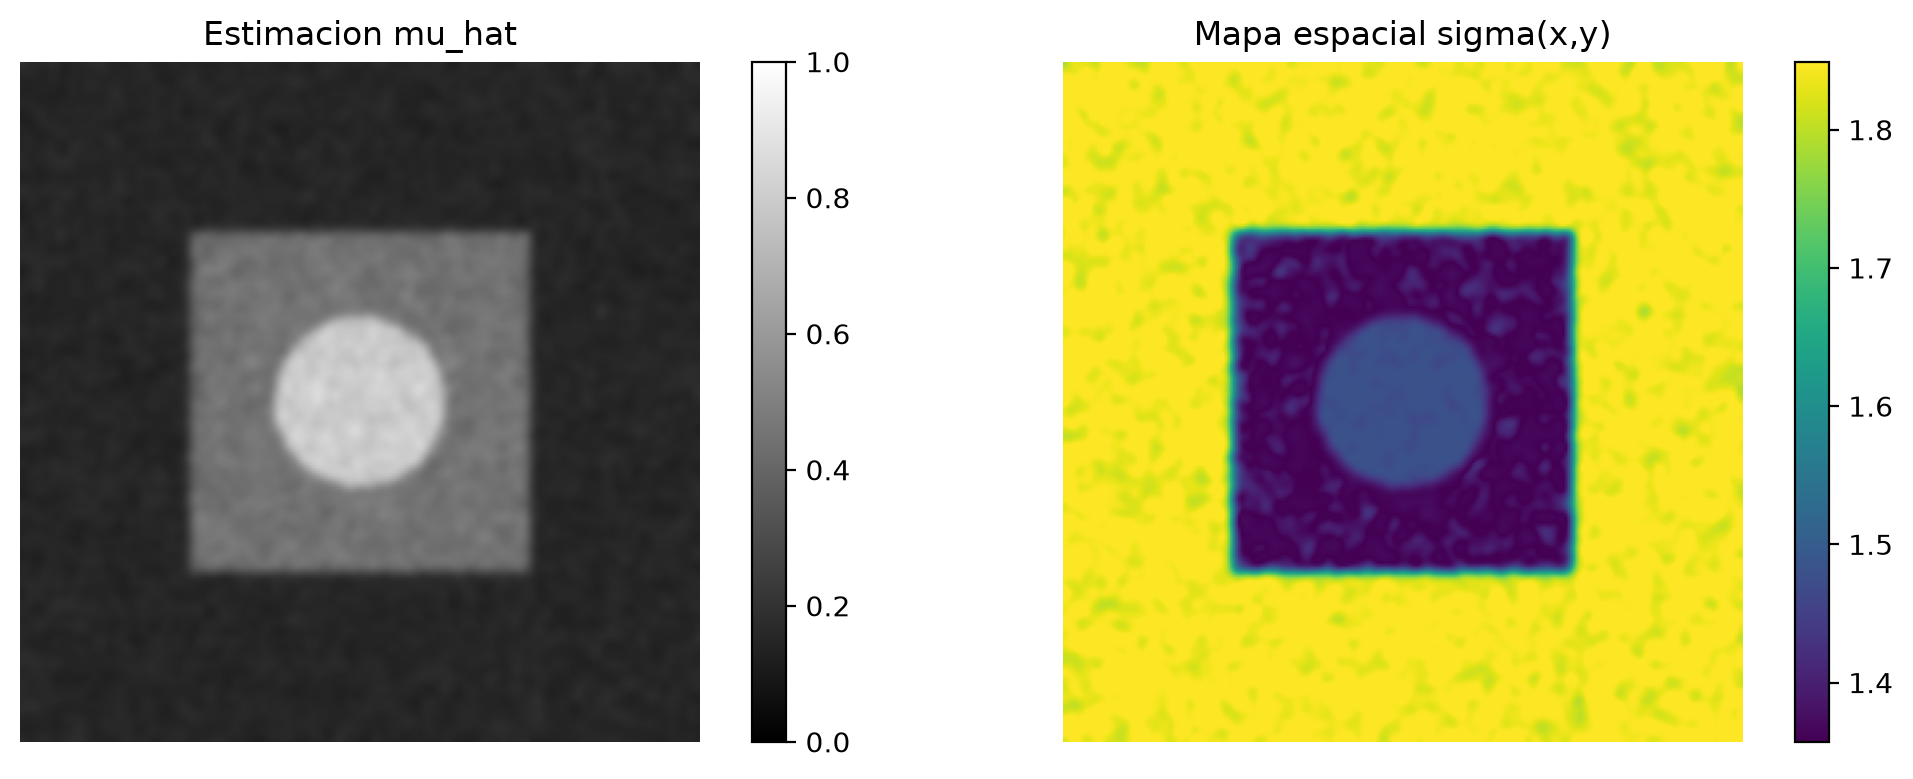
\includegraphics[width=0.82\textwidth]{pregunta_1/output/adaptativo_estimacion_muhat_mapa_sigma.png}
    \caption{Estimacion local $\hat{\mu}(x,y)$ y mapa utilizado de $\sigma(x,y)$.}
\end{figure}

La comparacion cuantitativa fue:

\begin{table}[H]
    \centering
    \begin{tabular}{lrrrr}
        \toprule
        Metodo & Global & Fondo & Cuadrado & Circulo \\
        \midrule
        Sin filtrado & 0.078170 & 0.061416 & 0.106228 & 0.143646 \\
        Mejor global & 0.024104 & 0.016884 & 0.036971 & 0.043401 \\
        Adaptativo & 0.024234 & 0.016884 & 0.036990 & 0.044789 \\
        \bottomrule
    \end{tabular}
    \caption{Comparacion de RMSE entre la imagen sin filtrar, el filtro global y el adaptativo.}
\end{table}

En esta realizacion, el mejor filtro global obtiene un RMSE ligeramente menor
que el adaptativo. El adaptativo asigna escalas diferentes segun la
intensidad, pero la estimacion suavizada de $\hat{\mu}$ y la interpolacion
pueden producir valores que no coinciden exactamente con el optimo de cada
region. Ambos metodos tienen practicamente el mismo error en el fondo.

\begin{figure}[H]
    \centering
    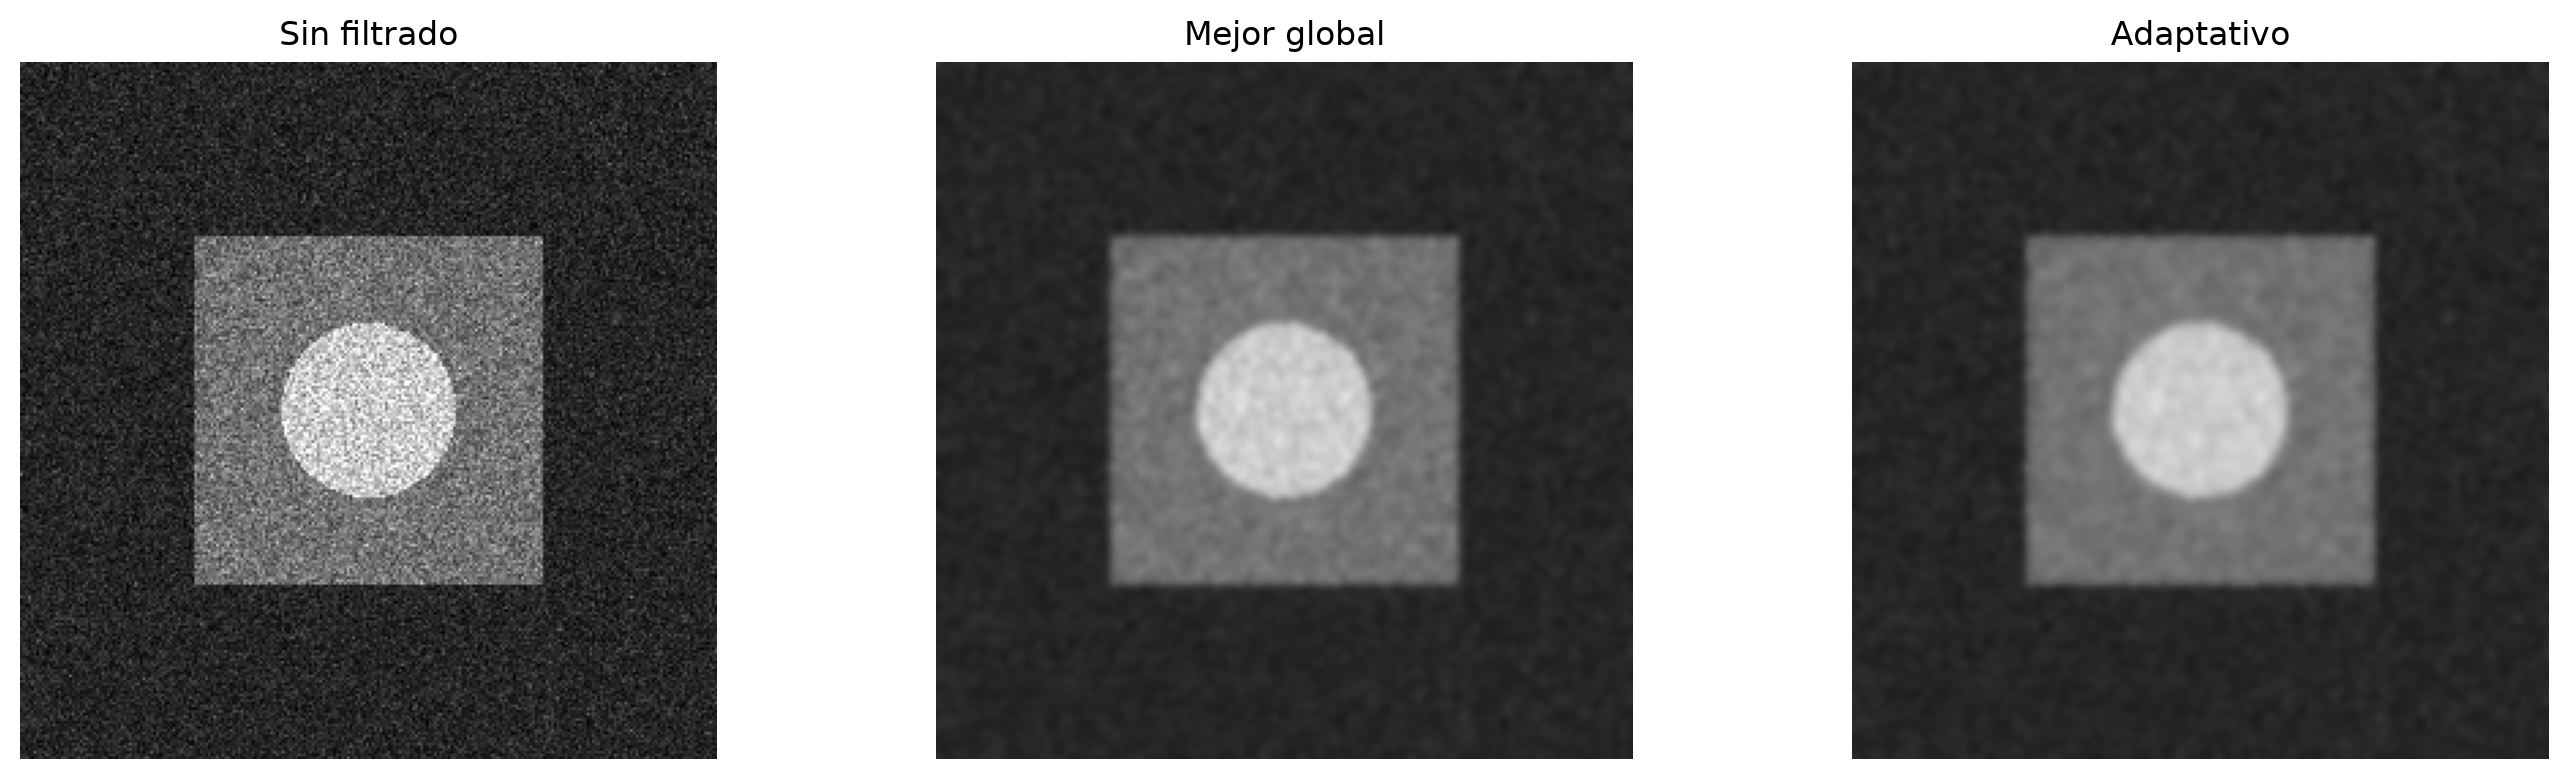
\includegraphics[width=0.9\textwidth]{pregunta_1/output/adaptativo_comparacion_resultados.png}
    \caption{Imagen ruidosa, mejor resultado global y resultado adaptativo.}
\end{figure}

\subsection{Analisis de fronteras}

El filtro adaptativo no puede escribirse, en general, como una unica
convolucion con un kernel fijo, porque el kernel depende de la posicion.
La implementacion que utilizo aproxima el resultado mediante un banco de
filtros Gaussiano y una mezcla espacial.

Un sigma grande reduce el ruido, pero tambien promedia intensidades de ambos lados
del borde. En este caso el suavizado auxiliar genera transiciones continuas
en el mapa de $\sigma$, por lo que no aparecen saltos ideales entre regiones.
Una modificacion simple para reducir aun mas los halos seria limitar el
sigma maximo cerca de bordes o incorporar un detector de bordes que evite
promediar intensidades de regiones distintas.

\begin{figure}[H]
    \centering
    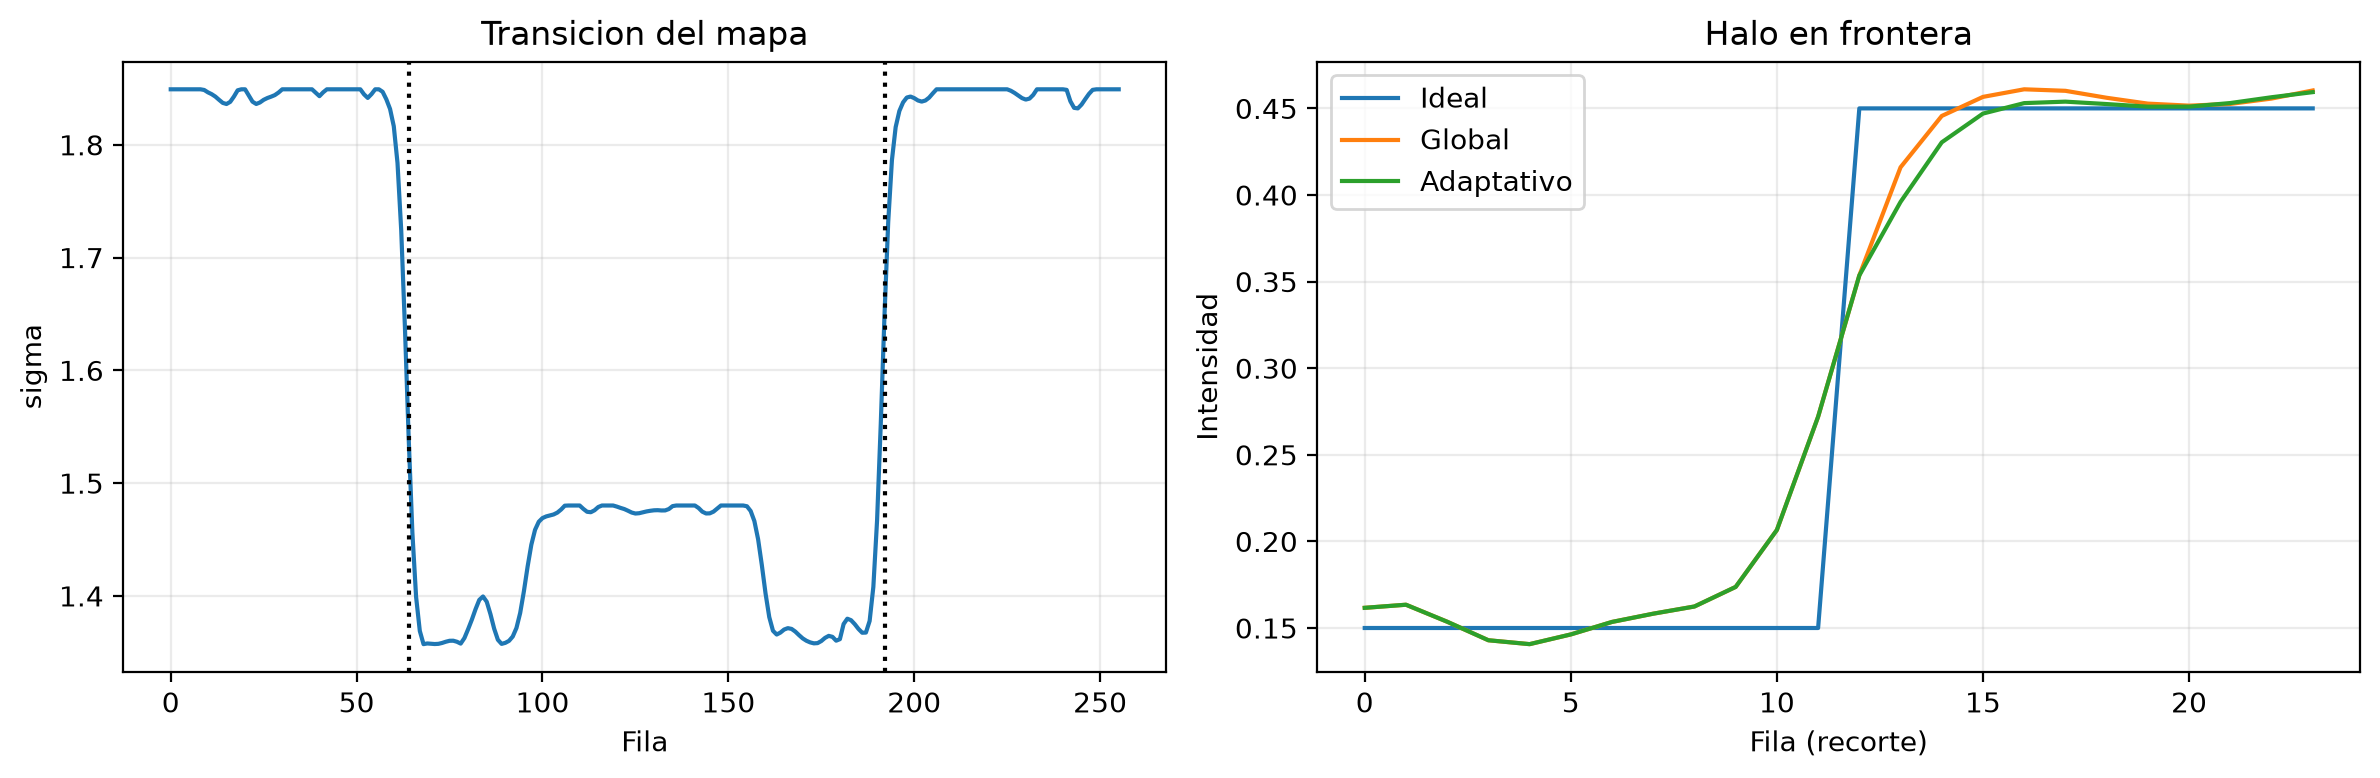
\includegraphics[width=0.88\textwidth]{pregunta_1/output/adaptativo_analisis_fronteras.png}
    \caption{Transicion de $\sigma(x,y)$ y comportamiento de los filtros cerca de una frontera.}
\end{figure}

\subsection{Preguntas guiadas}

\textbf{1) Varianza del ruido Poisson.}
Si $k\sim\operatorname{Poisson}(Nx)$, entonces
$\operatorname{Var}(k)=Nx$. Como $y=k/N$, se obtiene
\[
\operatorname{Var}(y)=\frac{x}{N}.
\]
Por esto, las regiones mas intensas presentan mayor ruido absoluto. El
filtrado debe equilibrar la reduccion de varianza con el sesgo producido en
las fronteras.

\textbf{2) Pixeles cercanos a los bordes.}
Se incluyeron porque permiten medir el efecto real del filtro sobre las
fronteras. Si se midiera solamente una zona plana y alejada de cualquier
borde, el sesgo por mezcla seria menor y el $\sigma$ optimo probablemente
seria mayor, ya que se podria suavizar mas sin desplazar una transicion.

\textbf{3) Tamano y normalizacion del kernel.}
El radio se obtiene como $r=\lceil3\sigma\rceil$, por lo que el kernel tiene
tamano $(2r+1)\times(2r+1)$. El soporte finito aproxima la mayor parte de la
masa de la Gaussiana y la normalizacion evita alterar el brillo de regiones
constantes.

\textbf{4) Obtencion de $\hat{\mu}$ y $\sigma(x,y)$.}
Se aplico un suavizado Gaussiano auxiliar de $\sigma=2$ sobre la imagen
ruidosa. Luego se interpolo entre los puntos determinados por los optimos
regionales. En pixeles interiores del fondo, cuadrado y circulo,
$\hat{\mu}$ es aproximadamente $0.15$, $0.45$ y $0.80$, respectivamente, y
los sigmas asociados son aproximadamente $1.849$, $1.357$ y $1.480$.

\textbf{5) Convolucion fija.}
No existe, en general, un unico kernel fijo porque cada posicion puede tener
un sigma diferente. Se puede aproximar usando varias convoluciones globales
y mezclando sus resultados, que es la estrategia utilizada.

\textbf{6) Comparacion de resultados.}
El filtro global fue levemente mejor en el RMSE total, en el cuadrado y en
el circulo. En el fondo ambos resultados fueron iguales a seis decimales.
La diferencia se explica porque el sigma global coincide con el minimo global,
mientras que el metodo adaptativo usa una estimacion local y una
interpolacion que suavizan la seleccion de parametros. El adaptativo sigue
siendo conveniente cuando la intensidad y el nivel de ruido cambian
espacialmente, aunque las fronteras pueden limitar su mejora.

\clearpage
\section{Pregunta 2}
\subsection{Datos e infraestructura de difusion}

Se utilizo la imagen ``cameraman'' en escala de grises, normalizada al
intervalo $[0,1]$. Luego se agrego ruido Gaussiano de media cero y desviacion
estandar $0.05$, usando una semilla fija. El RMSE de la imagen ruidosa fue
$0.04791$.

Selecciono dicha imagen porque la imagen mencionada en el enunciado no fue adjuntada, sin embargo la imagen ``cameraman'' es adecuada para este estudio porque
contiene regiones relativamente homogeneas, bordes definidos y variaciones
locales de intensidad.

\begin{figure}[H]
    \centering
    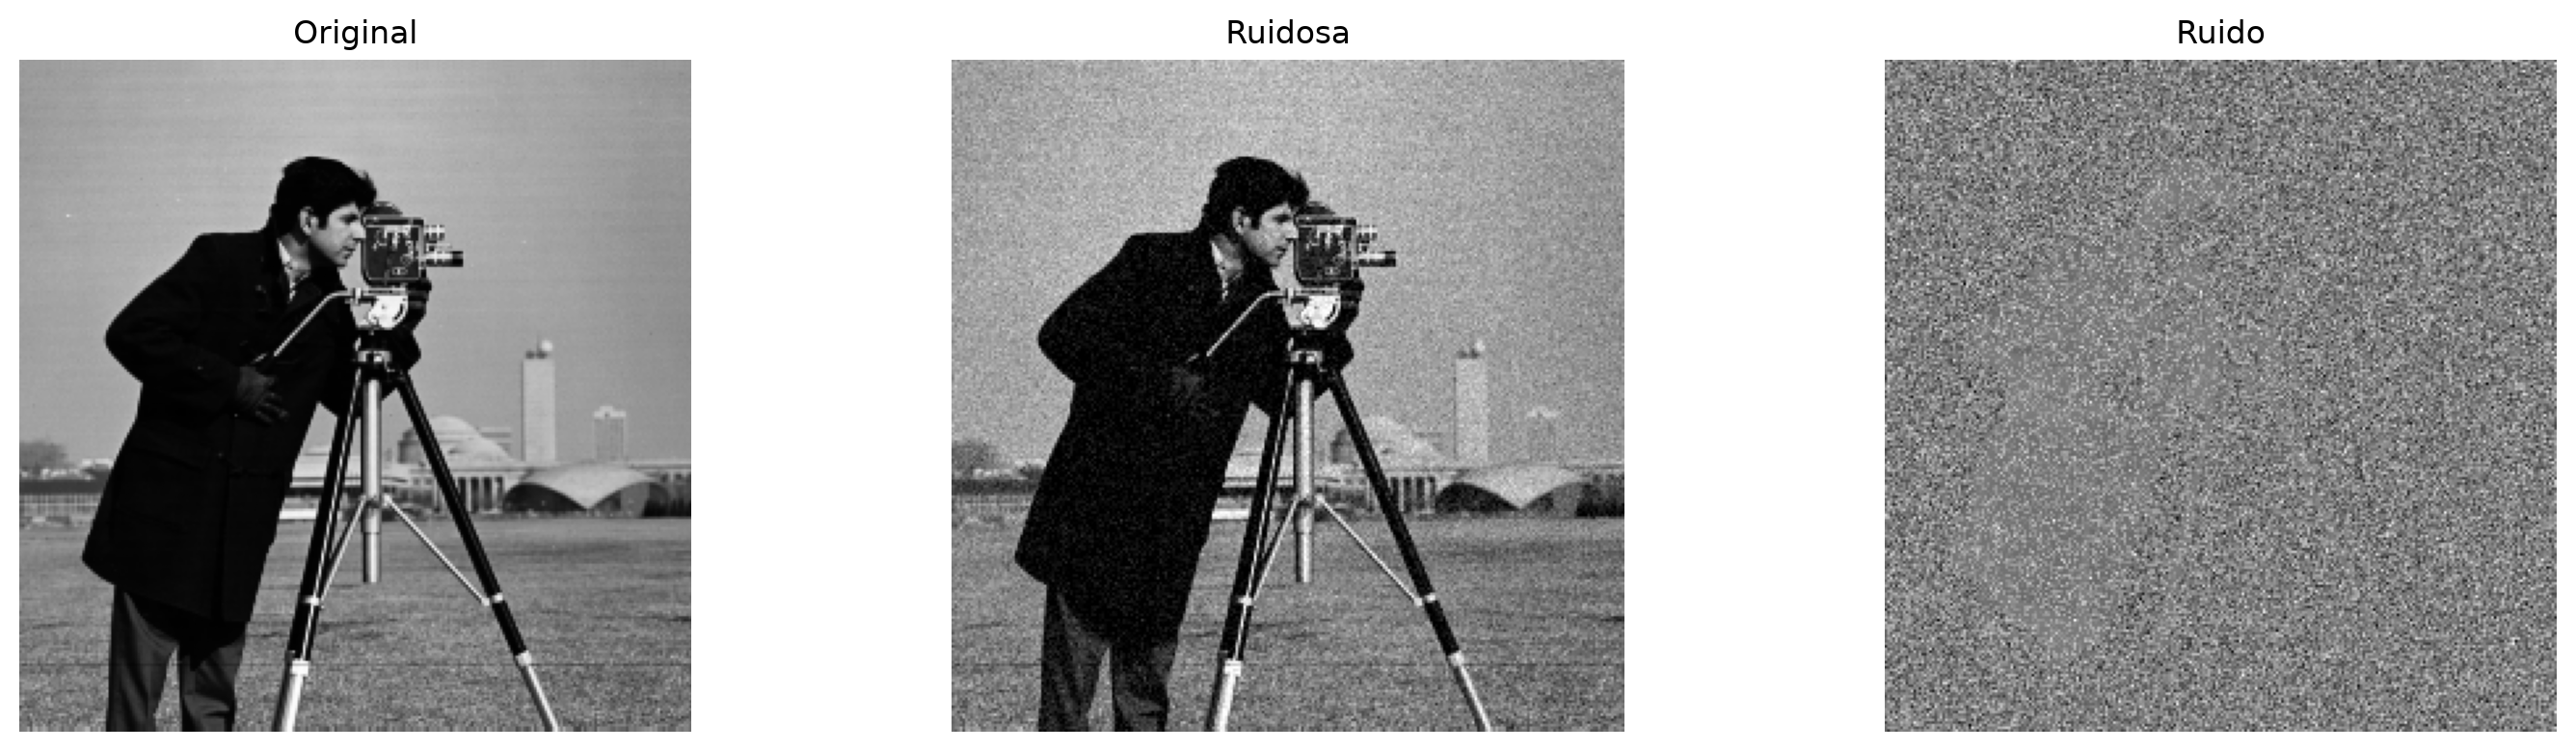
\includegraphics[width=0.92\textwidth]{pregunta_2/output/implementacion_datos_ruido.png}
    \caption{Imagen original, imagen ruidosa y ruido agregado.}
\end{figure}

Todas las variantes utilizan la misma actualizacion. En cada
iteracion se calcula el coeficiente sobre la imagen actual y se calculan los
flujos hacia los cuatro vecinos. Los coeficientes de las caras se obtienen
promediando los valores de los dos pixeles que comparten cada cara. La
actualizacion se limita a $[0,1]$.

El gradiente usa diferencias centrales y el Laplaciano usa el estencil de
cuatro vecinos. Para controlar la estabilidad se utilizo
\[
\lambda \leq \frac{1}{4\max(c)}.
\]
Cuando la opcion automatica esta activa, el programa reemplaza el valor
solicitado por el menor entre este limite y el valor pedido.

\subsection{Variacion Total y efecto de epsilon}

El primer coeficiente fue
\[
c_{\mathrm{TV}}=\frac{1}{\sqrt{|\nabla u|^2+\varepsilon^2}}.
\]
Se probaron $\varepsilon=0.005$, $0.02$, $0.08$ y $0.20$. Cuando el
gradiente es pequeno, el coeficiente es aproximadamente $1/\varepsilon$:
un epsilon pequeno produce mucha difusion en regiones planas, pero tambien
obliga a utilizar un paso temporal mas pequeno.

\begin{figure}[H]
    \centering
    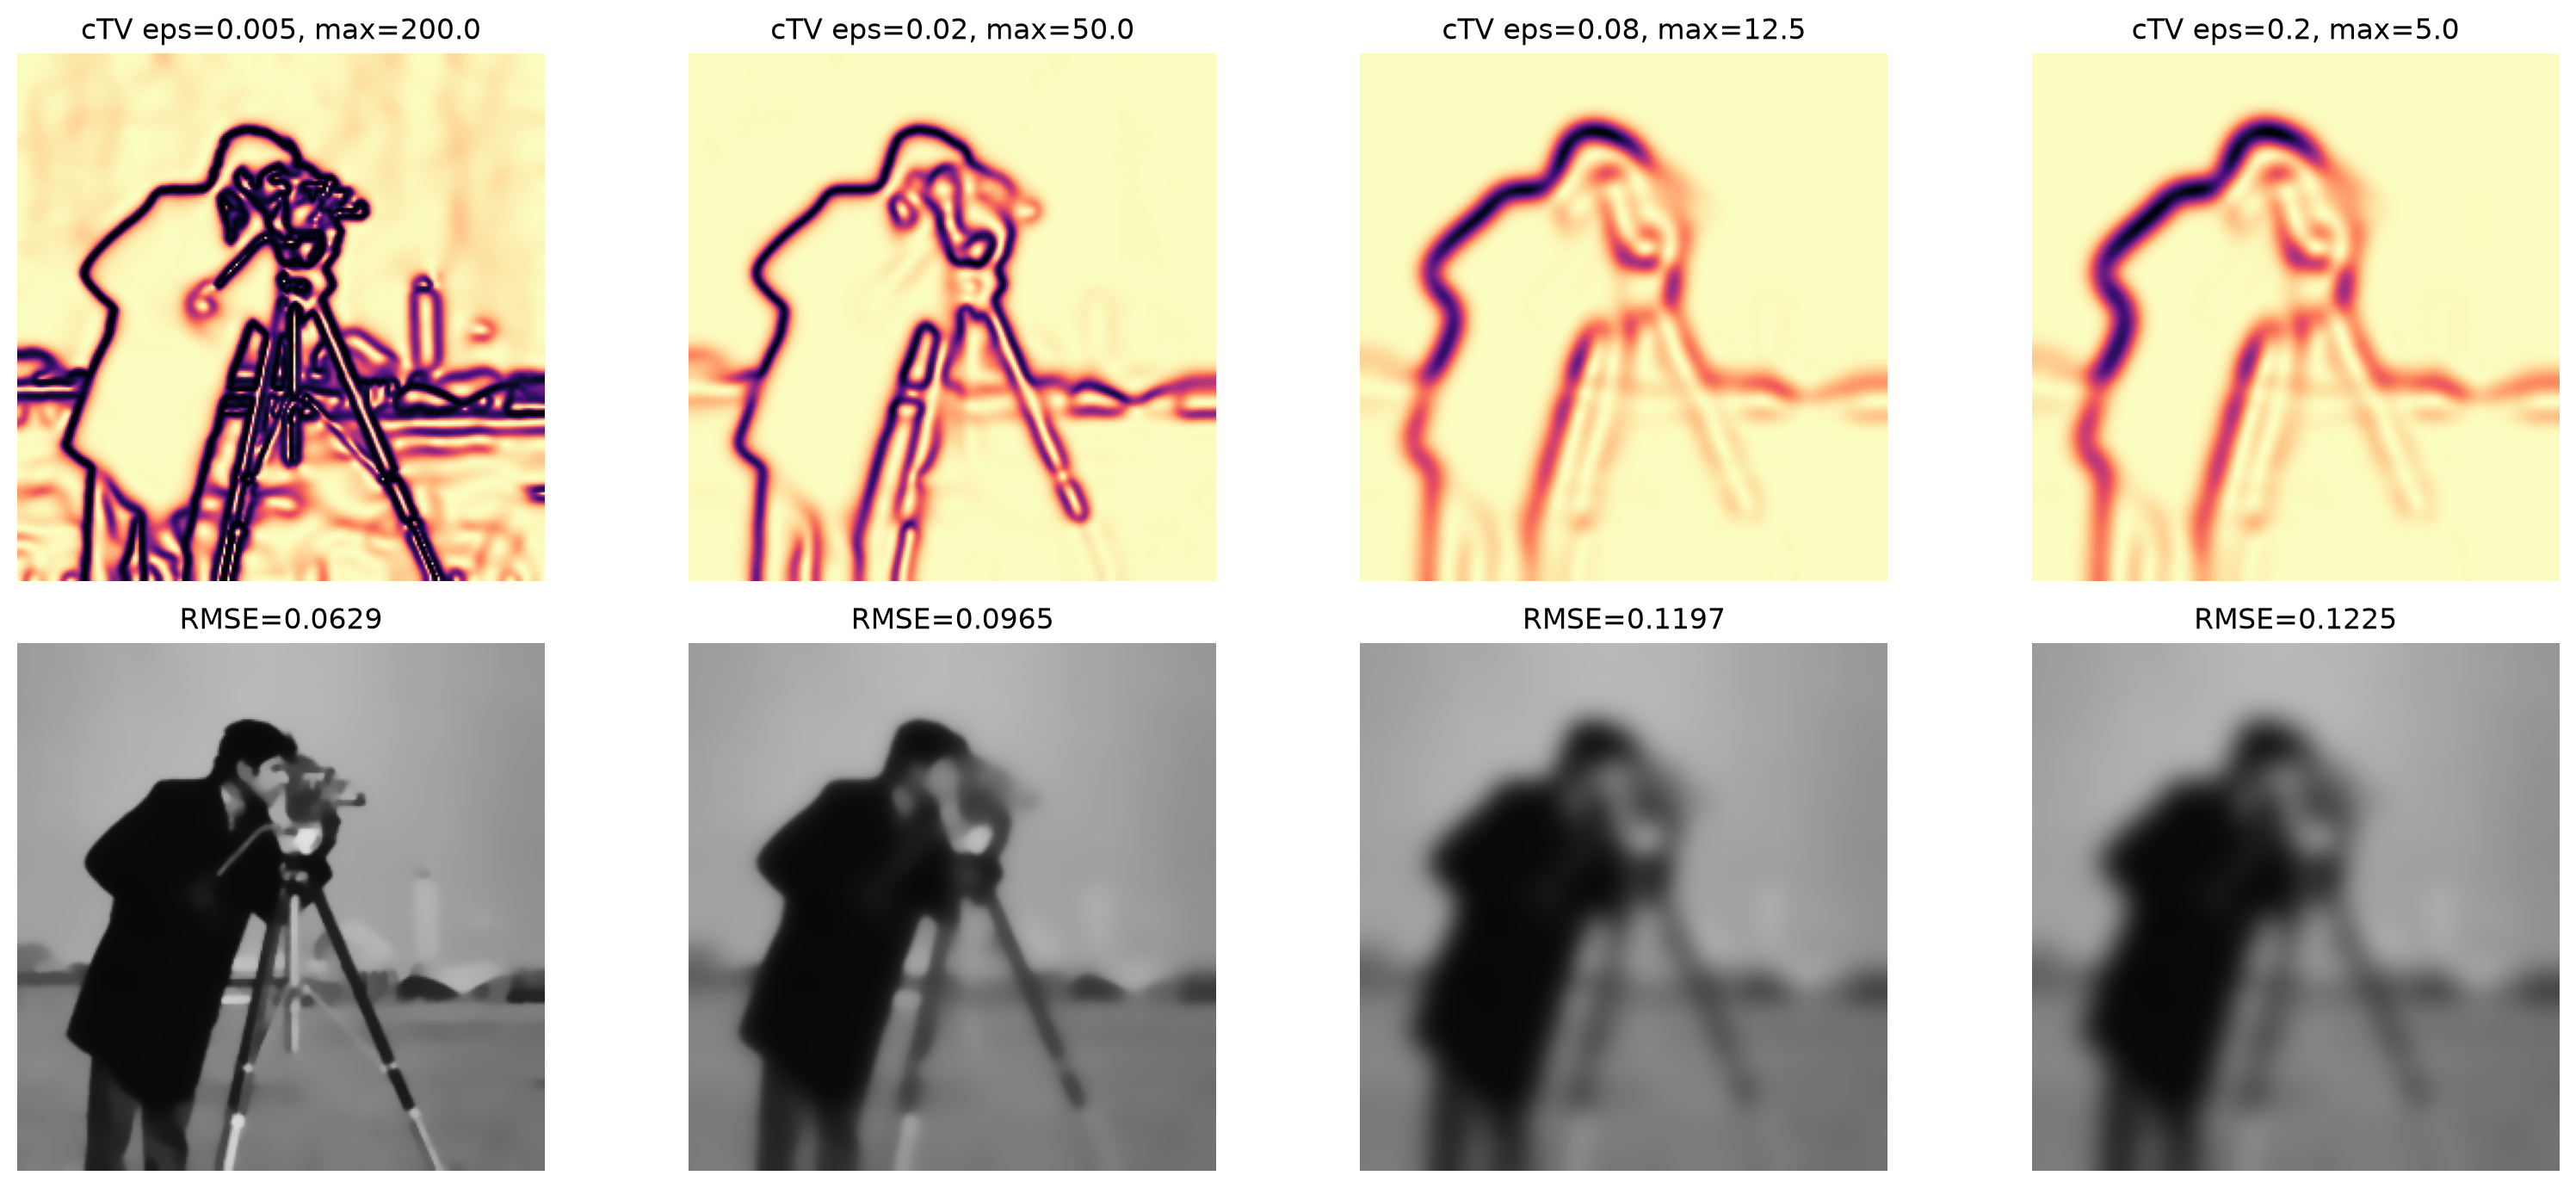
\includegraphics[width=0.95\textwidth]{pregunta_2/output/experimentacion_tv_sensibilidad_epsilon.png}
    \caption{Mapas de $c_{\mathrm{TV}}$ y resultados para distintos valores de epsilon.}
\end{figure}

Con $\varepsilon=0.005$, el maximo teorico del coeficiente es cercano a
$200$ y el limite estable es aproximadamente $0.00125$. Para
$\varepsilon=0.08$, estos valores son aproximadamente $12.5$ y $0.02$.
Por lo tanto, disminuir epsilon aumenta el contraste entre zonas que se
suavizan y bordes que se protegen, pero reduce la estabilidad disponible.

\subsection{Efecto de lambda e iteraciones}

Se compara una evolucion lenta, una eleccion razonable, un caso de
sobre-suavizado y un caso inestable. El caso inestable
$\lambda=0.20$ sin aplicar la correccion automatica, aunque el limite
estimado era cercano a $0.00125$. Su RMSE fue $0.56090$ y la imagen alcanzo
el rango completo $[0,1]$.

\begin{figure}[H]
    \centering
    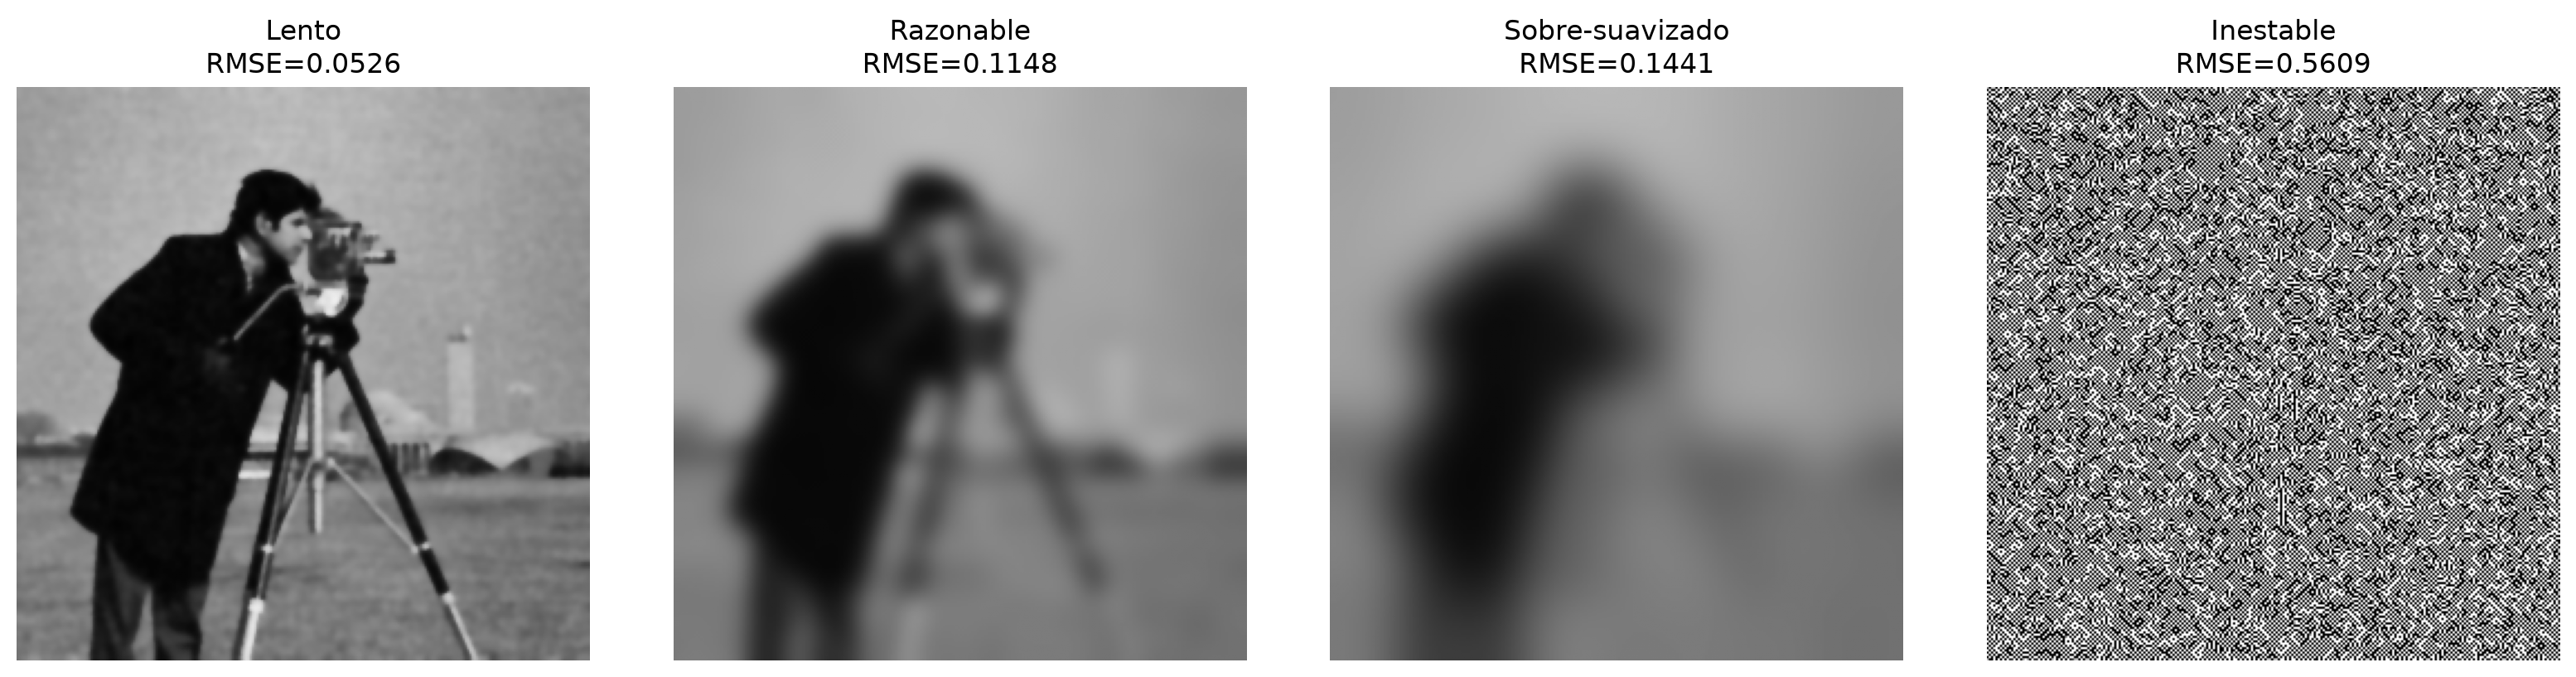
\includegraphics[width=0.95\textwidth]{pregunta_2/output/experimentacion_estabilidad.png}
    \caption{Efecto conjunto de epsilon, lambda e iteraciones.}
\end{figure}

\subsection{Coeficientes alternativos}

Se propusieron dos alternativas. La primera combina gradiente y Laplaciano:
\[
E=\left(\frac{|\nabla u|}{k_g}\right)^2+
\alpha\frac{|\Delta u|}{k_l},
\qquad c=\frac{1}{1+E}.
\]
La segunda agrega una medida de textura local:
\[
E=\frac{|\nabla u|^2}{k_g^2}
\,+\,\beta\frac{\operatorname{Var}_{3\times3}(u)}{k_v},
\qquad c=0.10+\frac{0.90}{1+E}.
\]

En ambos casos, cuando $E$ es pequeno la difusion es alta. Al crecer $E$,
el coeficiente disminuye y protege bordes o texturas. En la propuesta basada
en textura queda un piso de $0.10$, por lo que nunca se elimina por completo
la difusion.

\begin{figure}[H]
    \centering
    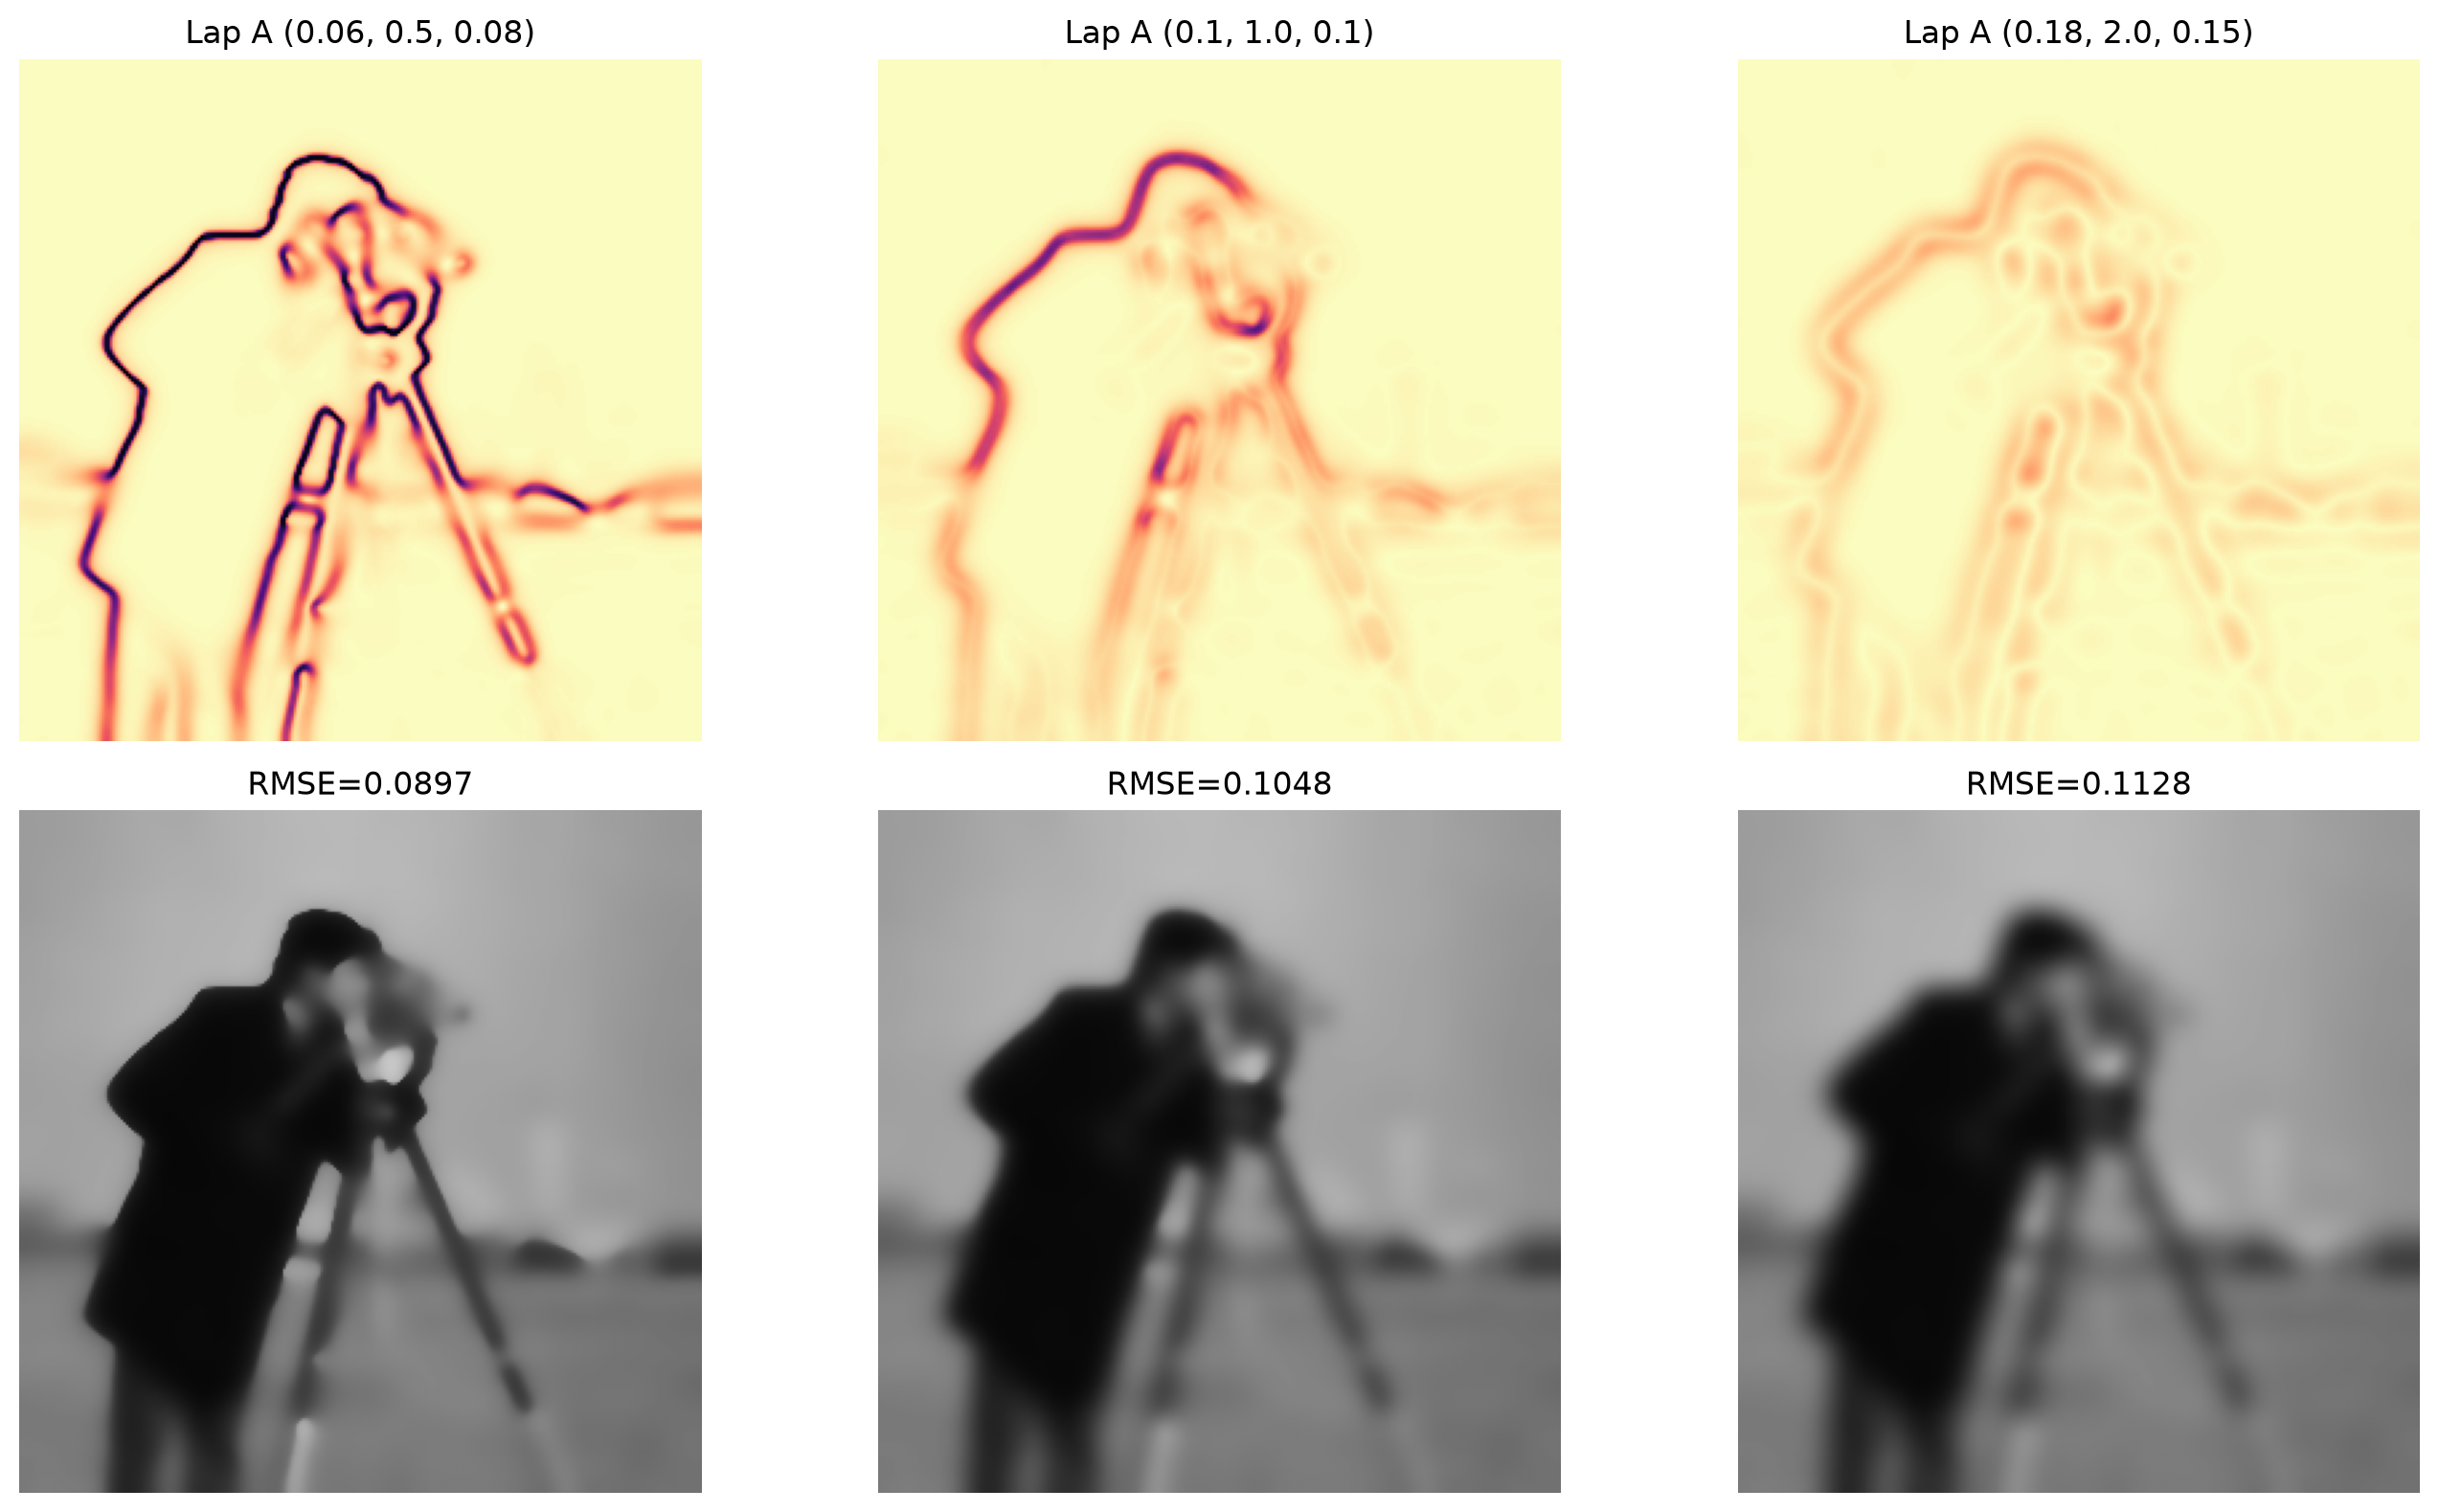
\includegraphics[width=0.95\textwidth]{pregunta_2/output/experimentacion_coeficiente_laplaciano.png}
    \caption{Exploracion del coeficiente que combina gradiente y Laplaciano.}
\end{figure}

\begin{figure}[H]
    \centering
    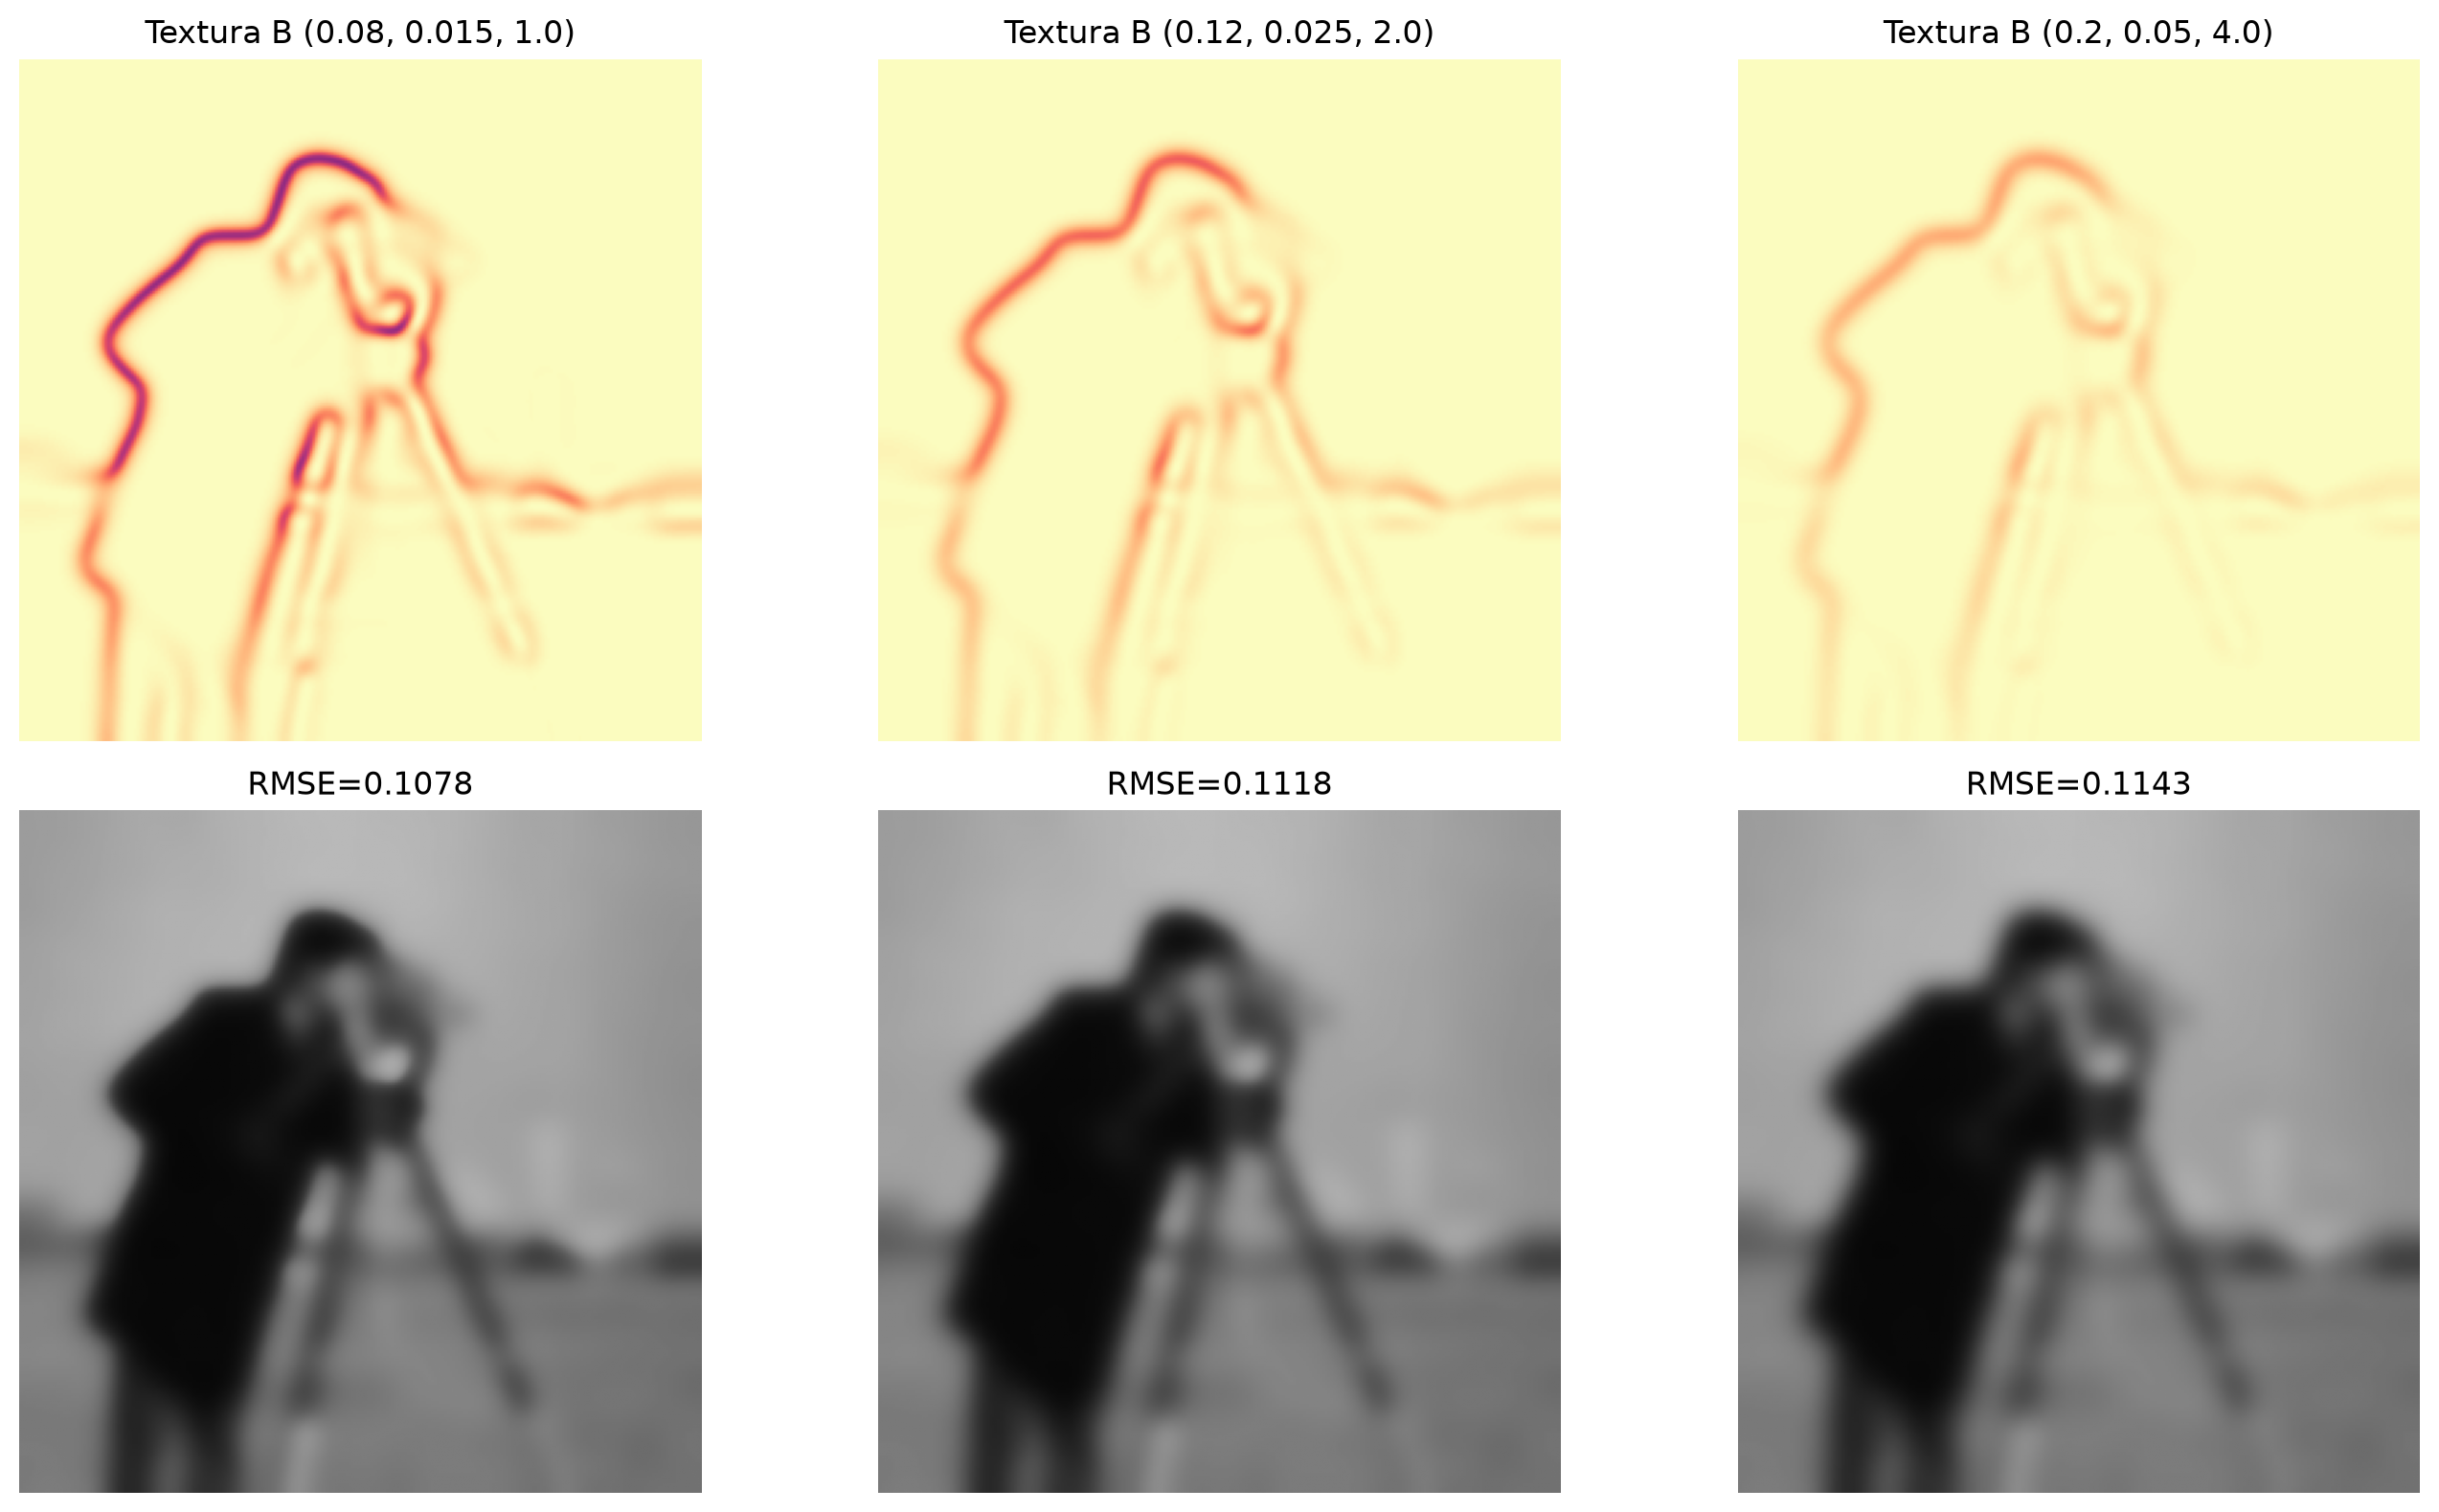
\includegraphics[width=0.95\textwidth]{pregunta_2/output/experimentacion_coeficiente_textura.png}
    \caption{Exploracion del coeficiente basado en gradiente y textura local.}
\end{figure}

\subsection{Sensibilidad del Laplaciano}

El Laplaciano agrega informacion de curvatura que no esta contenida
directamente en la magnitud del gradiente. Sin embargo, las segundas
derivadas son sensibles a variaciones rapidas producidas por el ruido. En
la imagen original la mediana de $|\Delta u|$ fue $0.02846$, mientras que
en la imagen ruidosa aumento a $0.16236$. El percentil 95 aumento de
$0.43191$ a $0.57121$.

Para controlar esta sensibilidad se utilizaron los parametros
`lap\_weight` y `lap\_scale`, que permiten limitar la influencia del
Laplaciano en el indicador $E$.

\begin{figure}[H]
    \centering
    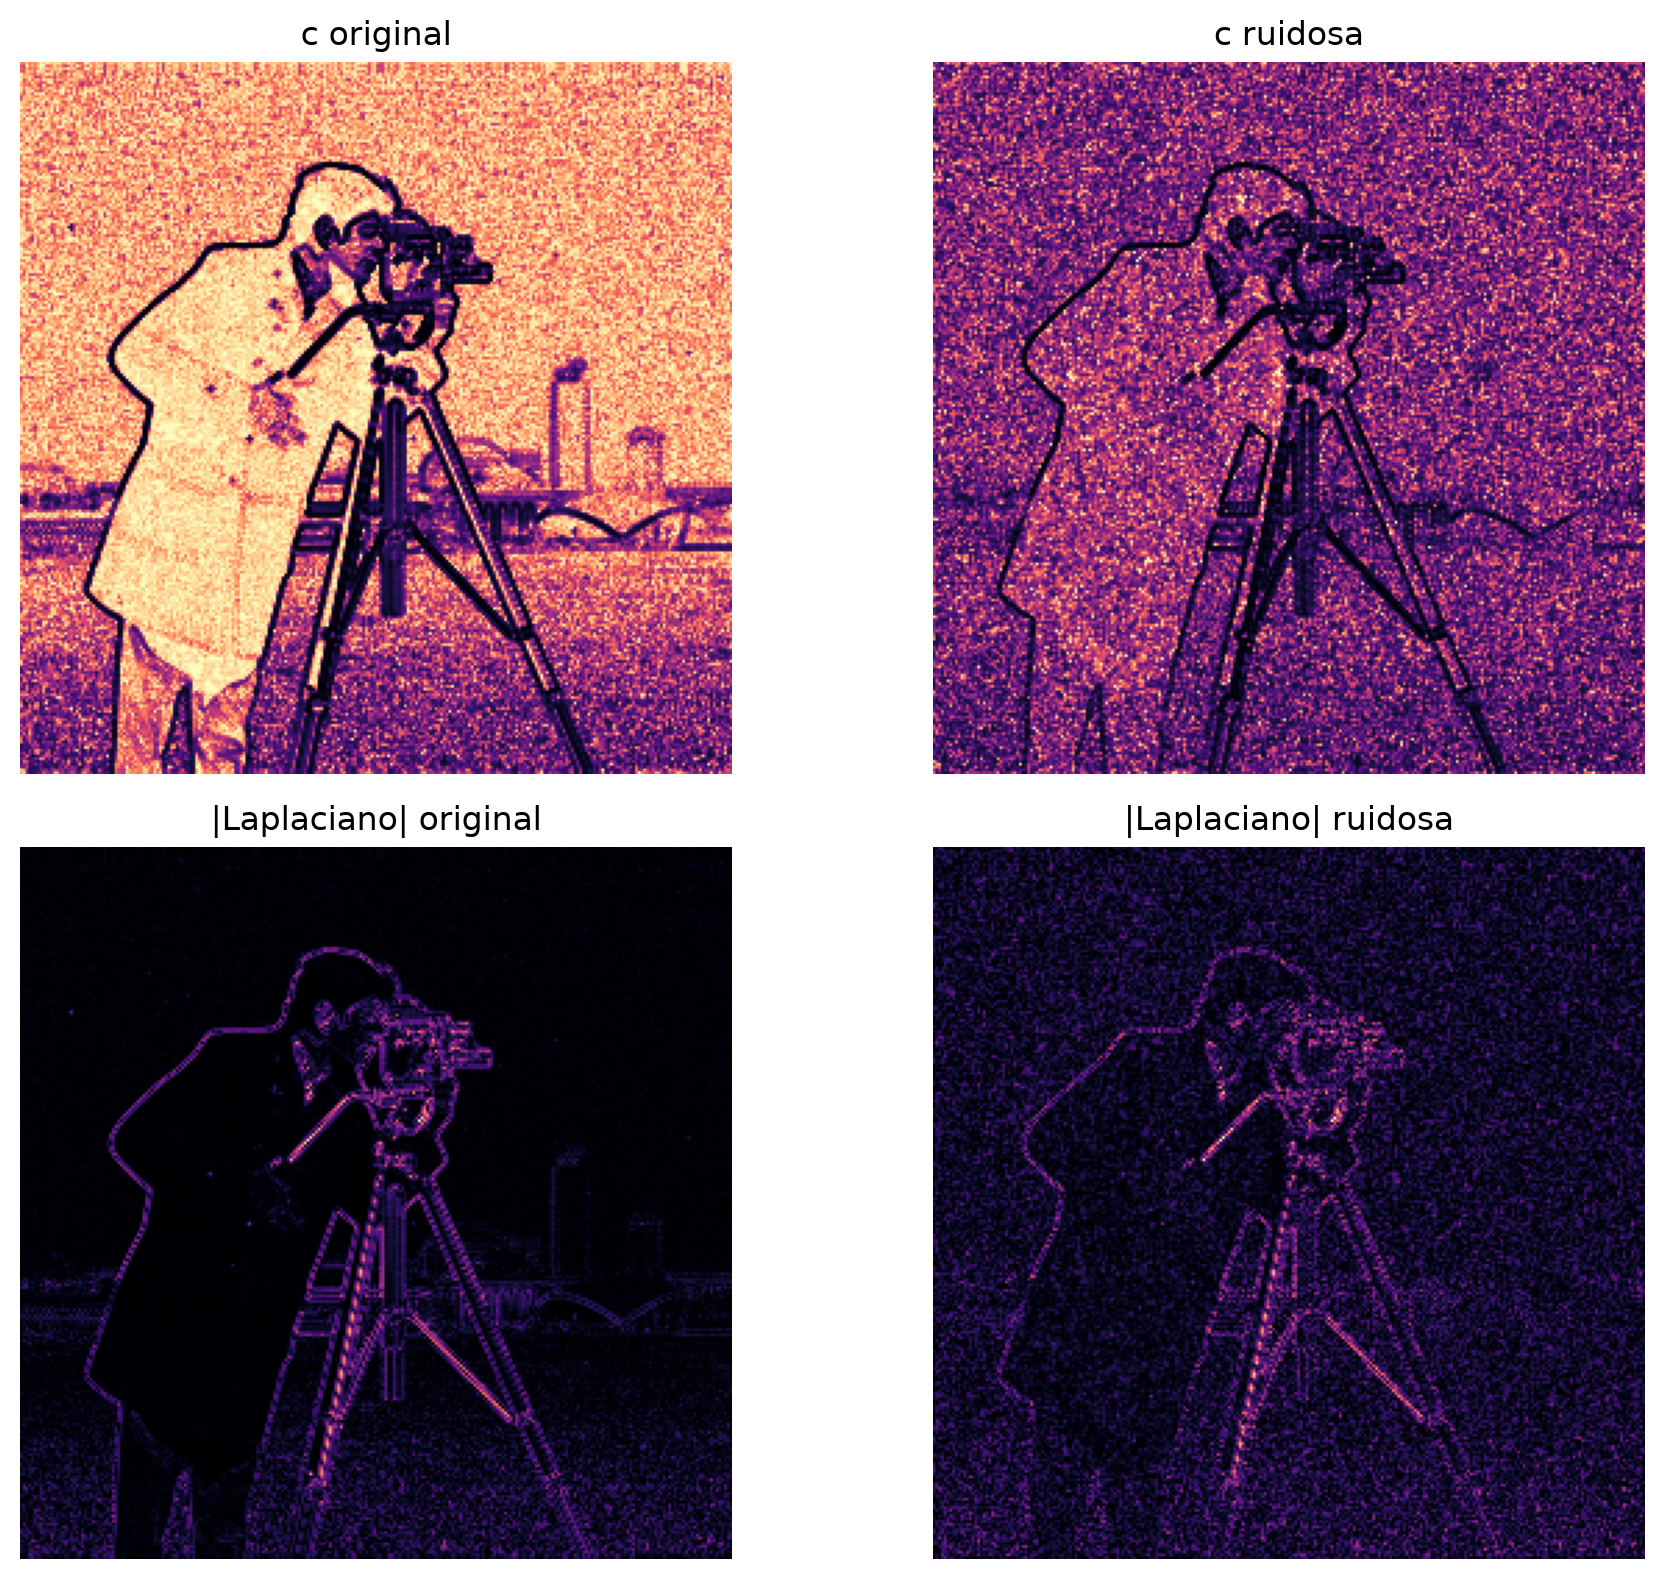
\includegraphics[width=0.75\textwidth]{pregunta_2/output/experimentacion_sensibilidad_laplaciano.png}
    \caption{Comparacion del coeficiente y del Laplaciano en imagen original y ruidosa.}
\end{figure}

\subsection{Comparacion final}

Para comparar los metodos se utilizaron diez iteraciones con parametros
ajustados de forma razonable. Los RMSE obtenidos fueron:

\begin{table}[H]
    \centering
    \begin{tabular}{lc}
        \toprule
        Metodo & RMSE \\
        \midrule
        Imagen ruidosa & 0.04791 \\
        TV, $\varepsilon=0.08$ & 0.06843 \\
        Lap A & 0.03860 \\
        Textura B & 0.05533 \\
        \bottomrule
    \end{tabular}
    \caption{Comparacion final respecto de la imagen original.}
\end{table}

En esta configuracion, Lap A obtuvo el menor RMSE. TV protege bien los
bordes, pero con pocas iteraciones no alcanza a reducir todo el ruido.
Textura B conserva informacion local y evita un suavizado excesivo, aunque
su reduccion de ruido fue menor. Lap A aprovecha la informacion de segunda
derivada, pero requiere cuidado porque el Laplaciano tambien responde al
ruido.

\begin{figure}[H]
    \centering
    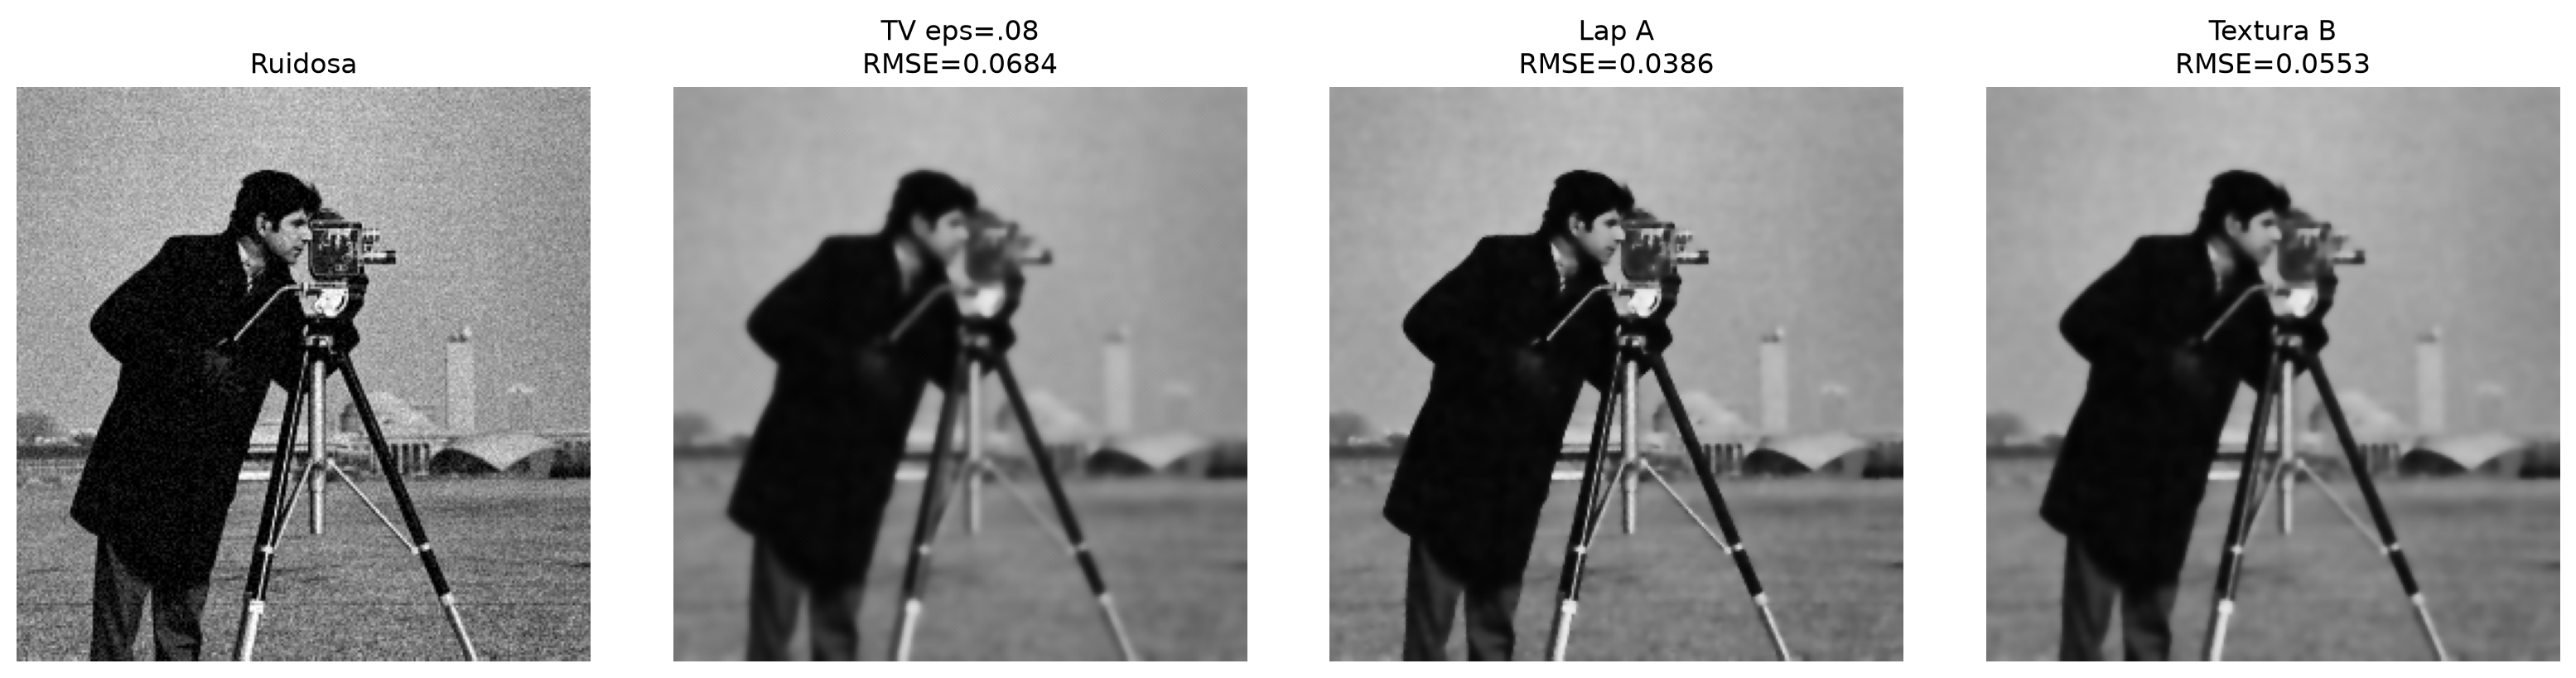
\includegraphics[width=0.95\textwidth]{pregunta_2/output/experimentacion_comparacion_final.png}
    \caption{Comparacion visual entre la imagen ruidosa y los tres metodos.}
\end{figure}

\begin{figure}[H]
    \centering
    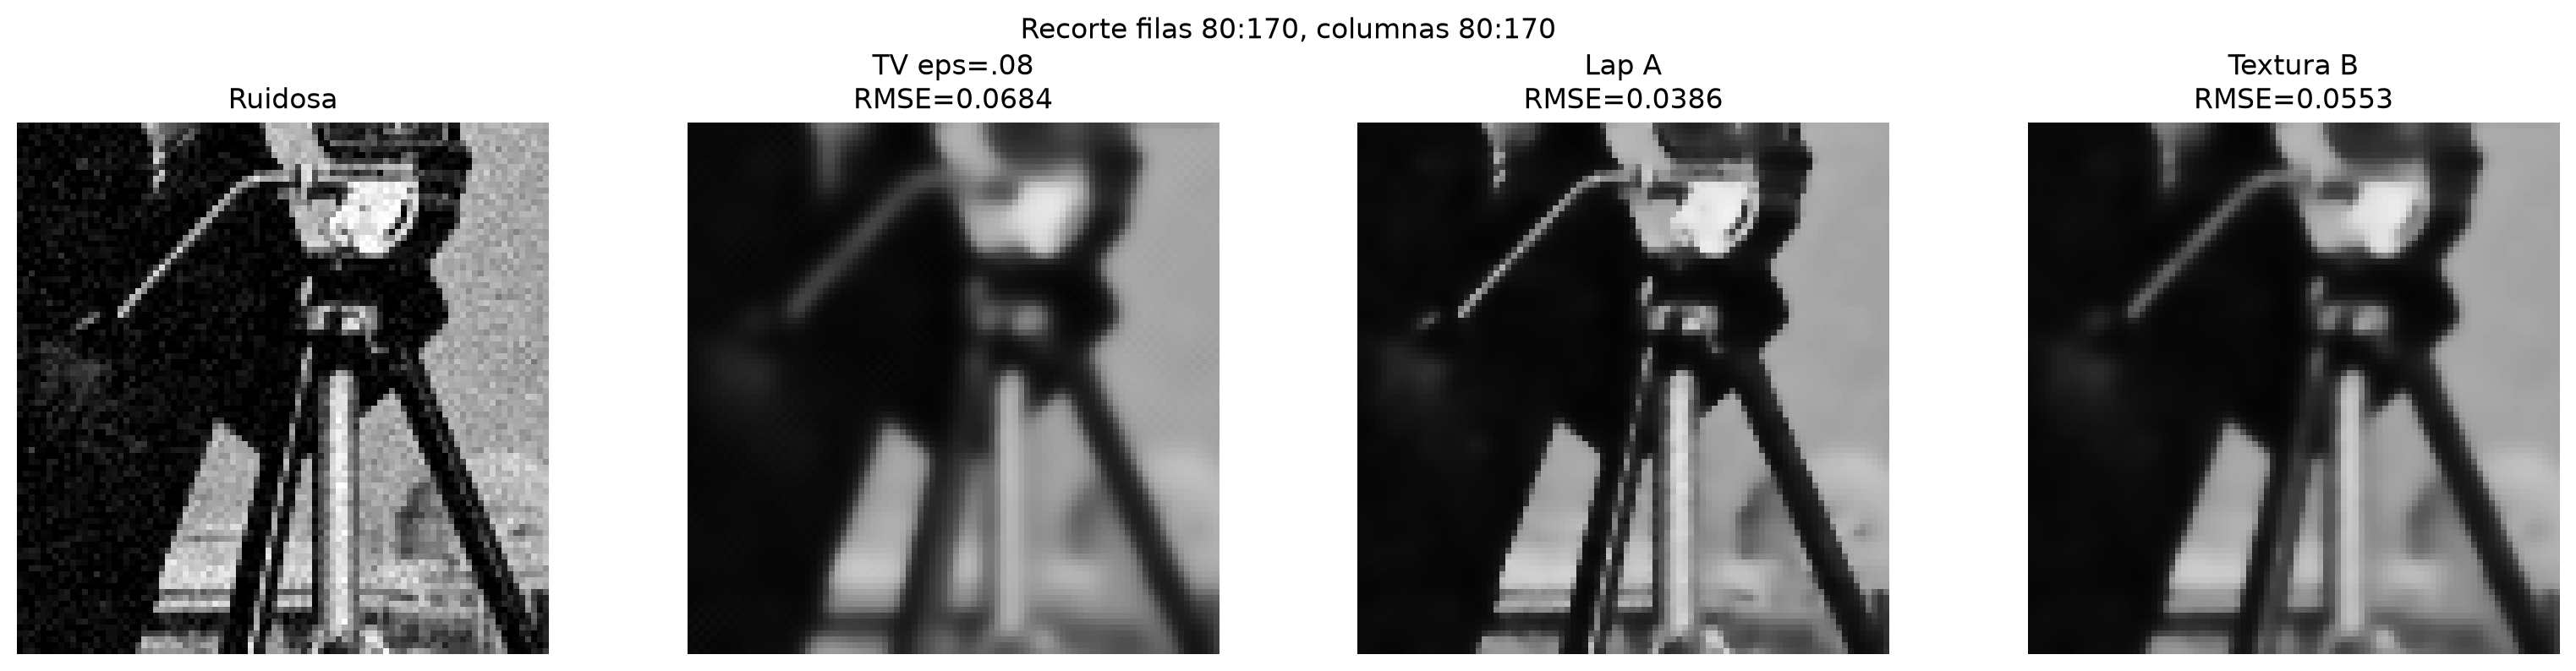
\includegraphics[width=0.95\textwidth]{pregunta_2/output/experimentacion_comparacion_recorte.png}
    \caption{Recorte ampliado para observar bordes y perdida de textura.}
\end{figure}

\begin{figure}[H]
    \centering
    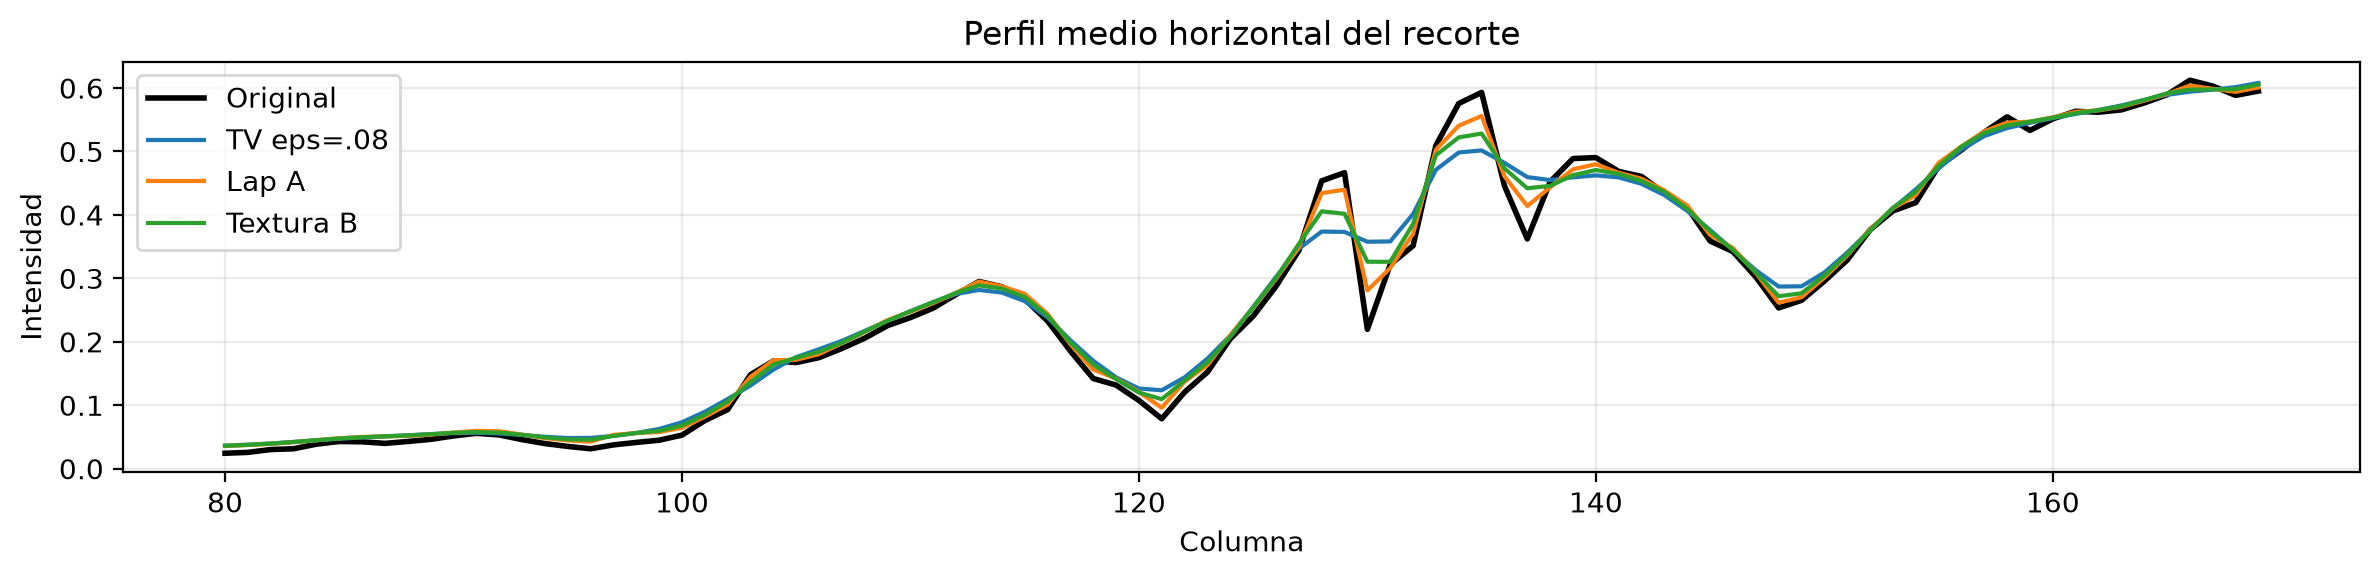
\includegraphics[width=0.9\textwidth]{pregunta_2/output/experimentacion_perfil_recorte.png}
    \caption{Perfil medio horizontal del recorte ampliado.}
\end{figure}

\subsection{Preguntas guiadas}

\textbf{1) Calculo en cada iteracion.}
El gradiente, el Laplaciano y el coeficiente se calculan sobre la imagen
actual $u$. TV usa el gradiente; Lap A usa gradiente y Laplaciano; Textura B
usa gradiente y varianza local. La actualizacion comun esta en la funcion de
difusion explicita.

\textbf{2) Papel de epsilon.}
Cuando $|\nabla u|$ es pequeno, $c_{\mathrm{TV}}\approx1/\varepsilon$.
Disminuir epsilon aumenta la difusion en zonas planas, pero tambien aumenta
$c_{\max}$ y reduce el lambda estable.

\textbf{3) Eleccion de lambda.}
Se estimo $c_{\max}$ con el maximo del mapa de coeficientes y se uso
$\lambda\leq1/(4c_{\max})$. Esta regla se aplica automaticamente salvo en el
caso inestable, que se dejo sin correccion para mostrar sus consecuencias.

\textbf{4) Comportamiento de $h(E)$.}
En ambas propuestas $c$ tiende a uno cuando $E$ es pequeno. Al aumentar
$E$, el coeficiente disminuye. En Lap A controlan la transicion $k_g$,
`lap\_weight` y `lap\_scale`; en Textura B la controlan $k_g$, $k_v$ y
`texture\_weight`.

\textbf{5) Informacion del Laplaciano.}
El Laplaciano detecta curvatura y cambios del gradiente. Su desventaja es
que amplifica el ruido, por lo que se regularizo su contribucion mediante
`lap\_scale` y `lap\_weight`.

\textbf{6) Actualizacion de dos pixeles.}
Con TV y $\varepsilon=0.08$, se obtuvo un pixel de gradiente bajo en
$(2,40)$, con $c=12.39337$. Sus diferencias Este, Oeste, Sur y Norte fueron
\[
(-0.06435,-0.08099,0.03586,0.02300).
\]
Su actualizacion con $\lambda=0.02$ fue $-0.01986$.

En el pixel de gradiente alto $(36,109)$ se obtuvo $c=3.31614$. Sus
diferencias fueron
\[
(0.01875,-0.02586,-0.61179,-0.03201).
\]
La actualizacion fue $-0.04131$. En ambos casos los flujos se ponderan con el promedio del
coeficiente entre el pixel central y su vecino.

\textbf{7) Coeficiente constante.}
Si $c$ es constante, todos los pixeles se difunden de la misma forma. El
metodo se convierte en difusion isotropica, que se relaciona con la ecuacion
del calor y, despues de varias iteraciones, con un suavizado Gaussiano. La
ventaja es la simplicidad, la desventaja es que tambien se suavizan bordes y
texturas.

\end{document}
\end{document}
